\section{Motivation}
The non-existent price recovery of the Western Canadian Select crude index since its collapse in 2015 has forced many Canadian energy companies to shift their operating strategies from expansion to optimization \cite{oil_price}.  Typically, existing processes in the oil and gas sector have been operating in a similar regime for many years.  In doing so, vast amounts of data have been collected for the current operating regime.  Through rapid advancements of computer hardware, this data can now be leveraged as a gold mine for modern data hungry machine learning algorithms.  Firstly, the data can be used for predictive applications such as forecasting, digital twinning, soft sensing, and even training purposes.  The data can also be leveraged to create ML-assisted safety applications similar to driver assistance in the automotive industry. For example, process monitoring and process forecasting ML models can be built to \textit{proactively} manage operational risk by identifying hazards well in advance of actual incidents. Modern optimal control methods (i.e., maximizing profits of a plant or minimizing operating cost) can also benefit greatly through the assistance of ML algorithms.  Currently, a common optimal control method in industry is model predictive control (MPC); however, the method assumes the availability of a (often times, accurate) process model.  In any industrial scale process, an accurate process model is nearly impossible to identify due to the vast amount of non-linear interaction effects.  Even after identification, the model would require re-tuning after several months due to process drifts and other changes. Furthermore, for large processes, the dimension of the states and actions may be too large for online optimization to be feasible. One field of study known as distributed MPC aims to solve this computational hurdle by decomposing the system into smaller sub-systems; however, distributed MPC performance is typically subpar compared to its centralized counterpart due to communication issues \cite{distributed_mpc}. Through RL, such large problems may be computationally feasible as a centralized algorithm by pre-computing the optimal control policies offline. Moreover, process drifts can be naturally handled by RL through its direct adaptive optimal control nature \cite{direct_adaptive}.  For traditional optimal control, adaptive characteristics are typically indirect and require re-identification of the system models.  In the case of RL, the policy is adapted directly through interactions with the environment. There exist numerous \textit{big data} machine learning success stories in the technology sector such as deep learning for highly effective targeted advertisement. However, applications involving highly complex and non-linear models in the process industry are still severely limited even though there exist large archives of data. One main reason for the absence of recent big data ML progress in the process industry is the lack of a workforce skilled in both ML \textit{and} process control.

Many technology companies and ML engineers specialized in the big data have attempted to fill the gap; however, process control data is exceedingly different compared to the typical user or transactional data used by technology companies. The data in process control is typically unintuitive and is ofte unreliable or noisy. As such, traditional ML engineers lacking engineering expertise will struggle to build models that translate to true value. Indeed, most of the effort in machine learning projects is not spent on the algorithms, but rather, the data pre-processing step.  That is, even simple algorithms such as linear regression can achieve neural network performance if the data is properly de-noised and the proper features are selected. Without fundamental engineering expertise, feature selection and data de-noising could be almost impossible. For example, an engineer trying to predict the heat released by a reaction would intuitively selects the mass and temperature features due to his/her knowledge of thermodynamics while a ML engineer would start with arbitrary initial features out of the thousands available. There also exist many time delays in chemical processes and feature engineering is difficult without proper fundamentals of process engineering. Comparatively, the data in the technology sector is often very intuitive and easy to understand.  For example, building a classification algorithm for facial recognition is easier to understand compared to predicting when a pump will fail.  The former only requires an image of the individual or some 3D spatial data corresponding to the individual's facial features. In the latter, there may be thousands of interactions affecting the ultimate outcome of the pump, most of which are impossible to identify through intuition alone. Due to these differences, engineers not specialized in the process sector faced great challenges when attempting to create value in the process industry.

More recently, there has been a surge of ML innovations made by research scientists and AI start-up companies catered towards the process industry.  However, most were never commercialized because the mentality between industry and the engineers is vastly different.  In industry, the ultimate objective is to create shareholder value through risk-managed products; it may be traditional methods or it can be ML.  For the research scientists, the focus is more on the elegance and novelty of the algorithm, regardless of the complexity. For industry, such algorithms are difficult to explain to a non-technical audience, have a high cost of ownership for the customer, and are difficult to understand without a team of subject matter experts (which themselves cost a significant amount of money).

Throughout this thesis, the main theme is to introduce easy, cost effective solutions that explicitly consider the following four customer focused values required for successful commercial products \cite{marketing}:
\begin{itemize}
    \item \textbf{Functional value:} Describes the overall usefulness of the product compared to other available products.  For example, a ML anomaly detection algorithm may be far superior compared to other methods if sufficient data is present.
    \item \textbf{Monetary value:} The cost savings generated from this product (e.g., amount of money saved through using an optimization algorithm or preventing a loss incident).  
    \item \textbf{Social value:} Ability for the product to enhance your brand or product awareness is especially important for sales focused enterprises.  For example, after an individual goes to Disneyland, they may tell many people how great it was without any incentive from Disney.  In the process industry, operators and/or engineers will recommend great products that helped them in their jobs and/or become more productive without external incentives.
    \item \textbf{Psychological value:} Ability to make the company feel superior compared to the competition.  For example, a firm may believe it has better chances at winning contracts if its products contain state-of-the-art ML technology needed for big data applications.
\end{itemize}
Ultimately, the goal is to create organic growth for the local industry through new, innovative ways. This thesis introduces novel techniques to cater machine learning to the local industry, ranging from commodities transportation to automation.

\section{Introduction to AI}
Artificial intelligence (AI) has set off a change in perspective in the various sectors around the globe, ranging from health care to manufacturing.  The previously arcane topic is now spreading wildly across countless academic and industrial minds alike. Quick progressions in computing power and declining prices in data storage combined with AI's self-learning abilities have transcended AI to become the go-to algorithm for many difficult worldwide problems such as natural language processing, predictive analytics, and computer vision.  PwC projected AI to contribute well over \$15 trillion USD to the global economy by 2030, while elevating GDP of local markets by 26\%  \cite{pwc}. Generally speaking, the field of AI is ever-expanding and contains many goals.

Figure \ref{fig:AIGoals} shows the six major goals of AI.  Out of all the goals, machine learning (ML) is currently the most influential topic in industry.  The field of ML can be described as the study that develops algorithms to give machines explicit abilities to learn different tasks without being pre-programmed to do so \cite{AI}.  ML can be further decomposed into supervised learning, unsupervised learning, semi-supervised learning (a combination of supervised and unsupervised learning), and reinforcement learning.

\begin{figure}[H]
    \centering
    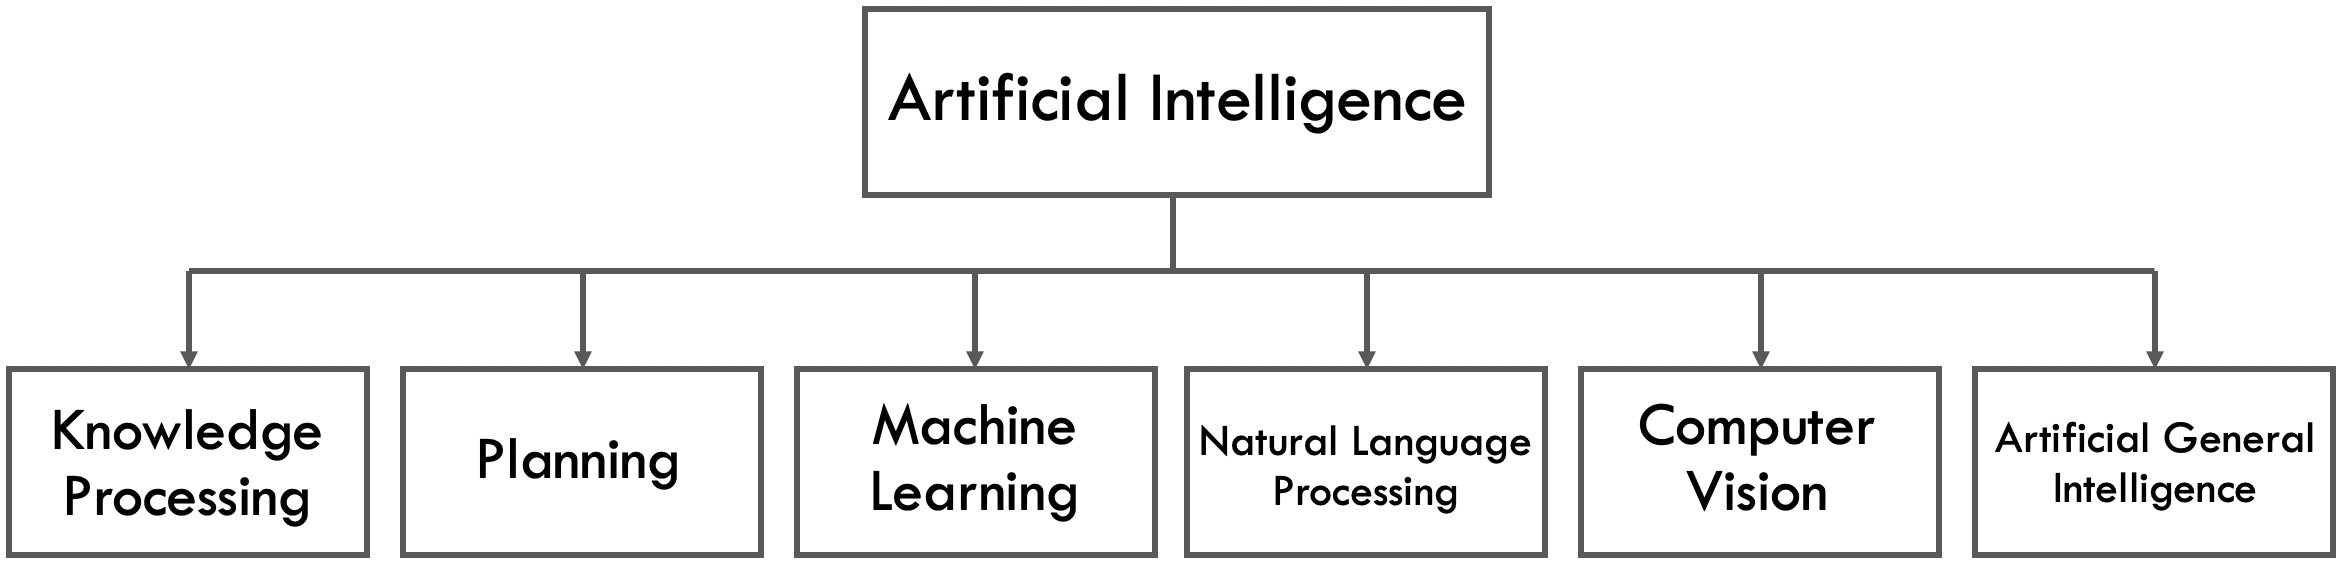
\includegraphics[width=\textwidth]{images/ch1/AIGoals.jpeg}
    \caption{The major goals of artificial intelligence.}
    \label{fig:AIGoals}
\end{figure}   

The sub-fields of ML are shown in Figure \ref{fig:MLGoals}.  In supervised learning, the algorithm learns the optimal input-output mapping, called the model, from a training data set pre-labeled by an external supervisor \cite{sutton}.  Be aware that not all labels provided are guaranteed to be correct. In fact, it is not uncommon to  have mislabeled data caused by noise in the original data set. For example, imagine trying to transcribe an interview with the audio playback heavily corrupted by noise.  In the process industry, the supervisor is typically a sensor measuring the current condition of the process (pressure, temperature, flow rate, etc.) and is often times unreliable. In the end, the performance of the supervised learning model is \textit{upper bounded} by the quality of the labels provided by the supervisor.  In the ideal case, the model can exactly replicate the right \textit{and wrong} labels of the supervisor. In unsupervised learning, the algorithms are typically used to optimally segregate data based on their similarity or to identify the principal components within large data sets \cite{Hinton, sutton}.  Objectively, unsupervised learning identifies hidden patterns within data sets through feature extraction and dimensional reduction. Semi-supervised learning is a hybrid between supervised and unsupervised learning where the models are trained on a small data set of labeled data and refined using features extracted from the unlabeled data set. For example, in the process industry, tasking an engineer to manually label data sets is a costly but required endeavor.  In many applications such as fault detection or root cause analysis, a well labeled data set is required to materialize any useful applications.  Using semi-supervised learning in these scenarios, the model can learn from the small labeled data set and extract additional helpful insights from the remaining unlabeled data to fine tune performance.  In this case, the final algorithm is vastly superior compared to its supervised or unsupervised learning counterpart \cite{machine_learning}.  Unfortunately, all the above methods exhibit one critical flaw: \textit{the inability to transcend the supervisor in terms of performance}. Although these methods may provide great cost reductions and/or greatly speed up production through automating trivial tasks, the methods fail to expand the current capabilities of modern methods.

\begin{figure}[H]
    \centering
    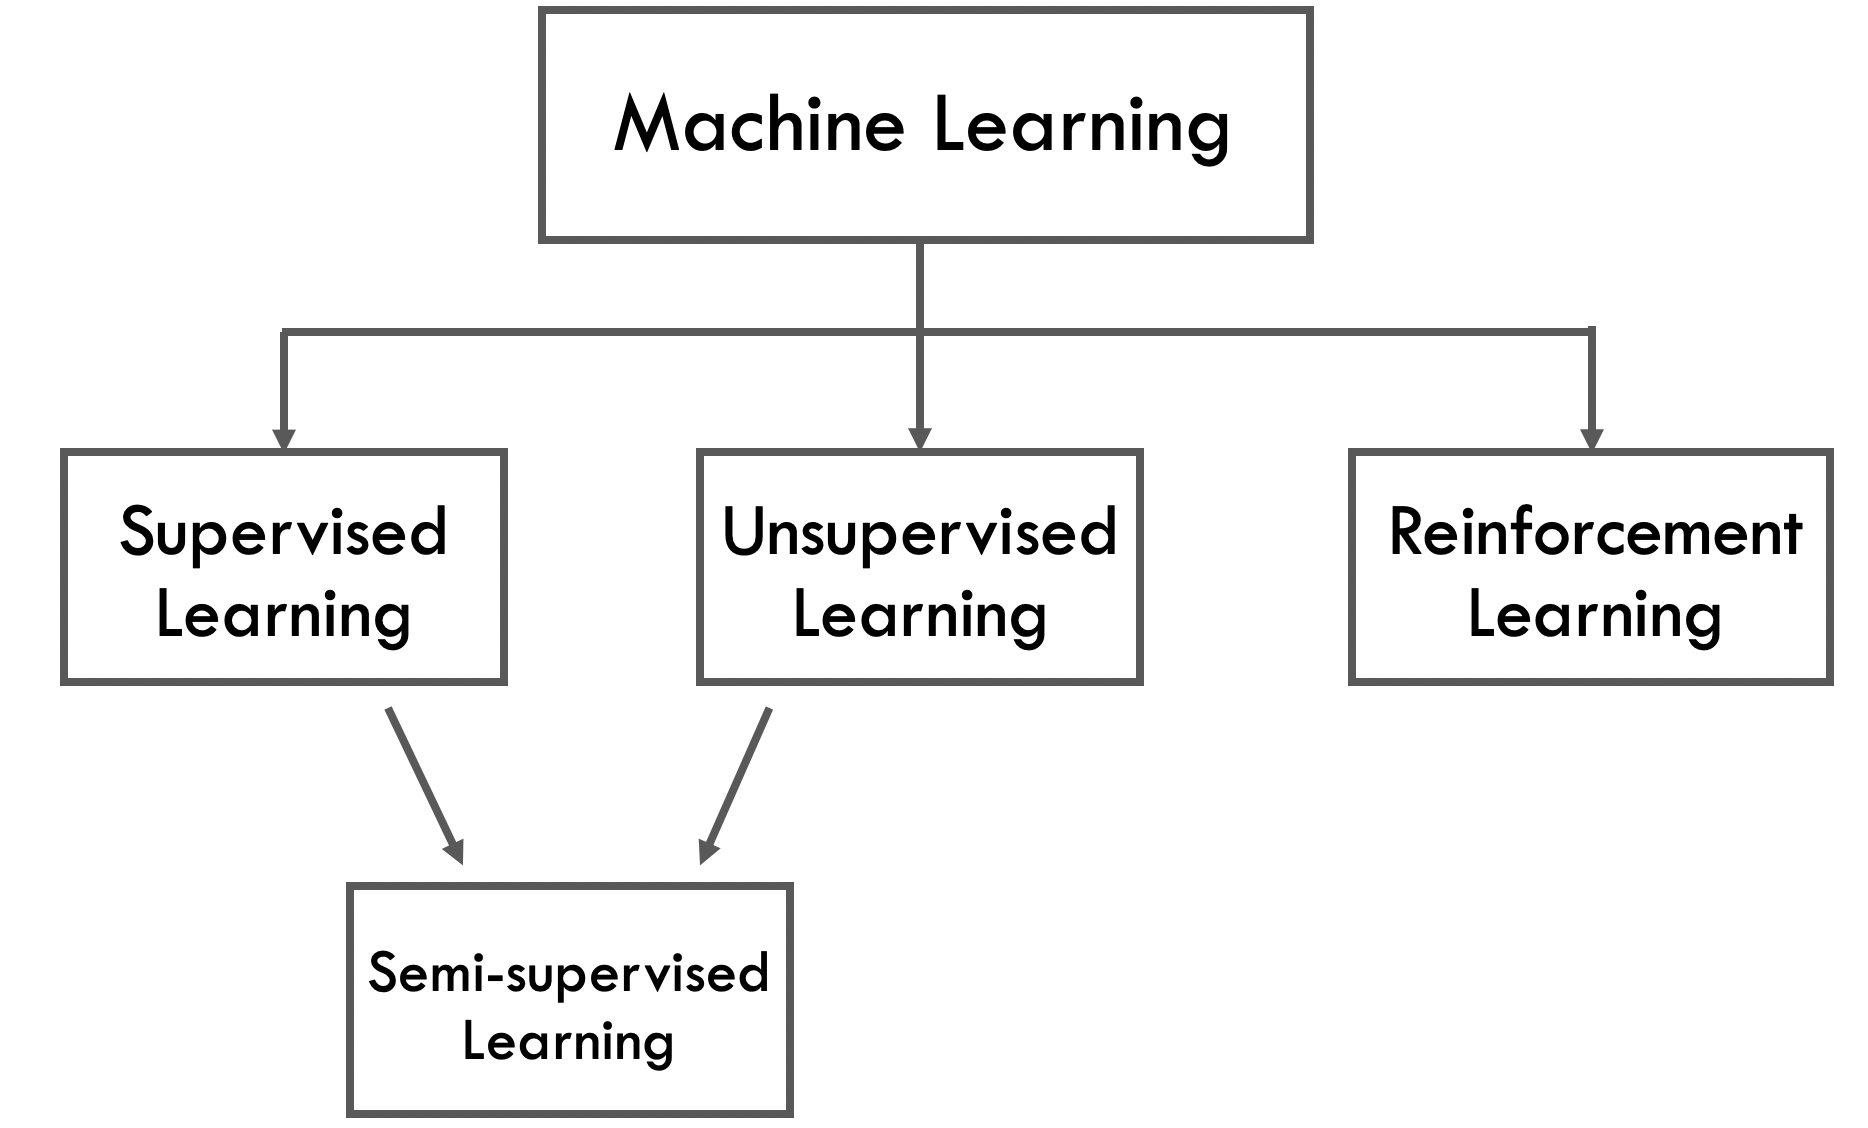
\includegraphics[width=0.6\textwidth]{images/ch1/MLGoals.jpeg}
    \caption{The sub-components of machine learning.}
    \label{fig:MLGoals}
\end{figure}   

Reinforcement learning (RL) aims to overcome this dilemma by providing machines the ability to \textit{surpass all known methods}.  More specifically, reinforcement learning \textit{agents} learn the optimal actions to perform in different situations (also called optimal policy) through self-interaction with the environment.  After each interaction, the agent is provided feedback via a scalar reward signal; large positive rewards follow good actions while negative rewards follow bad actions.  In challenging circumstances, actions affect both the immediate reward signal and the subsequent rewards there-forth. In an intuitively context, pursuing an University degree may yield negative immediate rewards; however, rewards years down the line may become significantly more positive due to the newly equipped knowledge.  These two characteristics---delayed feedback and guided trial-and-error search---differentiate RL from all other types of algorithms and ultimately permit RL to push the existing boundaries of known science \cite{sutton}.

\section{Thesis Outline and Contributions}
The thesis is organized as follows: First, basic concepts of RL and MPC will be introduced.  In Chapter 3, applications of ML algorithms in prediction applications will be explored on an industrial pipeline.  Following that, ML for process safety applications will be shown in Chapter 4. Safety applications include topics such as anomaly detection, anomaly prediction, and alarm management. Up until Chapter 4, the projects will mostly use traditional supervised, unsupervised, and semi-supervised learning methods because the applications are predictive in nature.  Towards the end of Chapter 4 until the end of the thesis, RL methods will be introduced because these applications are more control oriented. Chapter 5 contains various different RL applications in process control. Applications here include the optimal control of a waste water treatment plant, set point tracking control of small scale systems, and fault-tolerant control of an industrial distillation tower. Additionally, RL is also compared to MPC on simple small-scale systems in this chapter. Finally, this thesis is concluded in Chapter 6.  A comprehensive project report for the pipeline optimization project introduced throughout this thesis is shown in Appendix A.

The contributions of this thesis are as follows: In Chapter 3, methods for identifying representative process models in an industrial settings are introduced. Additionally, a new adaptive modelling method was formulated here to significantly reduce the cost of ownership of the machine learning models for the industrial partner. The adaptive method also overcomes catastrophic interference and can be retrofitted onto all model structures. Chapter 4 introduces novel data pre-processing approaches to anomaly detection and prediction in the process industry.  Additionally, a new RL-powered alarm management method is introduced for filtering of nuisance alarms, alarm reduction, and alarm prioritization.  Chapter 5 provides various comparisons between traditional optimal control methods and RL on many different systems. Furthermore, a new easy-to-implement continuous non-linear RL method is also shown here.  The last contribution in Chapter 5 is the extension of RL into a fault-tolerant control where RL is used for both the fault detection algorithm and the fault tolerant controller. Chapter 6 provides a literature review of all the renowned applications of RL as well as RL agents that have potential to materialize value in a process control environment.


% %%%%%%%%%%%%%%%%%%%%%%%%%%%%%%%%%%%%%%%%%%%%%%%%%%%%%%%%%%%%%%%%%%%%%%%%%%%%%%%%%%%%%
% % Bandits
% %%%%%%%%%%%%%%%%%%%%%%%%%%%%%%%%%%%%%%%%%%%%%%%%%%%%%%%%%%%%%%%%%%%%%%%%%%%%%%%%%%%%%

% %%%%%%%%%%%%%%%%%%%%%%%%%%%%%%%%%%%%%%%%%%%%%%%%%%%%%%%%%%%%%%%%%%%%%%%%%%%%%%%%%%%%%
% Bandits
%%%%%%%%%%%%%%%%%%%%%%%%%%%%%%%%%%%%%%%%%%%%%%%%%%%%%%%%%%%%%%%%%%%%%%%%%%%%%%%%%%%%%

\section{Preliminaries to Reinforcement Learning}

Reinforcement learning is a goal-directed learning algorithm which continually improves its own performance through interactions with the environment \cite{sutton}. The main objectives of reinforcement learning are to identify hidden structures within the environment and to find the optimal policy (i.e., optimal state to control action mapping) through guidance from an internal scalar reward (feedback). Two distinct characteristics that deviate reinforcement learning from other methods are its trial \& error search to find the optimal policy, and its ability to identify delayed reward signals. Modern reinforcement learning methods combine principles of optimal control and learning methods together to solve for the optimal control trajectory in an environment.  In the remaining sections of this chapter, fundamental reinforcement learning concepts will be introduced.  Then, tabular based RL methods will be shown.  However, due to the curse of dimensionality of high dimensional problems, tabular based approaches struggle in large multi-variate scenarios.  To overcome these issues, deep neural networks will be leveraged for function approximation, and deep reinforcement learning will be introduced.

\subsection{A Historical Overview}
Reinforcement learning is a combination of two fields of research: \textbf{optimal control} through extremizing an objective function through dynamic programming and \textbf{animal psychology} inspiring trial-and-error search. Originally, the \textbf{optimal control} problem was proposed for designing controller to maximize or minimize the objective function of a dynamical system over time \cite{mpc}.  By the 1950s, Richard Bellman extended on the works of Hamilton and Jacobi to develop a novel approach to solve the optimal control problem.  This approach, known as dynamic programming, optimizes a system's input trajectory by using the functional equation (a function where the unknowns are also functions) generated from the system's state information together with a value function \cite{bellman1}.  The functional equation, now called the Bellman equation, is mathematically represented as:
% Will leave spaces during submission for reviewers
\begin{equation}
    V(x) = r(x) + \gamma \sum P(x' | x, u) \cdot V(x')
    \label{eq:bellman_eq}
\end{equation}
where $V(x)$ represents the value function of $x$. Here, $\gamma$ denotes the discount factor to incorporate future uncertainty. $r(x)$ is the reward signal obtained as a function of the system's desired performance. $P(x'|x, u)$ is the dynamics function describing the transitional probability of arriving at state, $x'$, given $x$ and $u$. $V(x')$ is the value function of $x'$. Intuitively, the value function describes how good or how bad being in particular state is, assuming optimal behaviour thereafter; high values represent good states and low values for bad.  True dynamic programming is cursed by dimensionality (i.e., computational cost increases exponentially with the dimensions of the states and actions); thus, approximate dynamic programming (ADP) methods were developed to bypass this hurdle \cite{adp}.  In reinforcement learning, many ADP methods are leveraged to solve for the optimal policy. The concept of a feedback oriented learning system in RL originated from \textbf{animal psychology}. More specifically, the original concept was introduced in the early $20^{th}$ century, named the \textit{Law of Effect}. The law stated that animals tend to repeat actions resulting in good outcomes, vice versa for actions with bad outcomes \cite{thorndike}. Initially, the agent explores the environment in which it exists to identify the outcomes corresponding to different actions, then only repeating the actions resulting in good outcomes thereafter. By unifying dynamic programming from optimal control and trial-and-error search from animal psychology, the modern field of RL was developed. For a more comprehensive overview of the history of RL, see \cite{sutton}.

The development of RL is shown in Table \ref{tab:RLevo}.  Reinforcement learning takes its roots from the \textit{k}-armed bandit problem that has been extensively studied in engineering, psychology, and statistics.  This problem disregards state information, and only worries about solving the optimal actions for \textit{one} specific situation \cite{thompson1, thompson2, robbins, bellman_bandit}.  As a natural extension, Barto, Sutton and Brouwer expanded the idea to multi-situation systems \cite{bartosuttonbrouwer} through associative search, also known as \textit{contextual bandits}. The main objective of this algorithm was to find an optimal policy, $\pi^*(x)$, for each situation.  However, it only concerns the immediate rewards and not the long term consequences. Reinforcement learning was then developed to find the optimal policy for different situations based on immediate reward and the onward trajectory there-forth.  

\begin{table}[H]
\caption{From left to right, the evolution of reinforcement learning.}
\centering
\begin{tabular}{c|c|c}
\textbf{$k$-armed bandits}	& \textbf{Contextual bandits}	& \textbf{Reinforcement learning}\\
\hline
Optimal action		  & Optimal action			& Optimal action \\
One situation		  & Many situations			& Many situations \\
Immediate consequence & Immediate consequence	& Long-term consequence \\
\end{tabular}
\label{tab:RLevo}
\end{table}

\subsubsection{\textit{k}-armed Bandit}

The \textit{k}-armed bandit problem provides the fundamentals to understanding modern reinforcement learning.  Here, an agent is present and must choose action $u$ from $\mathcal{U}$, where $\mathcal{U}$ has $k$ choices.  After each action, a scalar reward from a stationary distribution will be returned to the agent as feedback. Favorable actions yield positive rewards, while unfavorable actions return negative rewards. The objective of the agent is to ultimately maximize reward over $N$ steps.  For each action, there is an expected reward called \textit{value}, given by Equation \ref{eq:01value}.

\begin{equation}
    \centering
    q_*(u) = \mathbb{E}[R_t | U_t = u]
    \label{eq:01value}
\end{equation}
where $u$ is the action taken at time, $t$.  $R_t$ is a scalar reward returned to the agent after action $u$ was performed at time $t$. $R_t$ is drawn from a stationary distribution, $R_t \thicksim N(q_*(u), \sigma^2)$. Finally, $q_*(u)$ is the expected reward of taking action, $u$.

The real value is unknown, however, an estimation can be computed and is denoted as $Q_t(u)$.  Given all $Q_t(u)$ is maintained, at any time, one $Q_t(u)$ will be greater than all others. Picking the action that corresponds to the maximum $Q_t(u)$ is known as \textit{greedy}, and the agent is said to be \textit{exploiting}.  If a non-maximum action is picked, the agent is \textit{exploring} \cite{sutton}.

Action selection based on estimating the value of actions are called \textbf{Action-value methods} \cite{action_value_method}. At time $t$, the estimate of the value is given by Equation \ref{eq: value_est} \cite{sutton}.

\begin{equation}
    \centering
    Q_t(u) = \
    = \frac{\sum_{i=1}^{t - 1} R_i \mathbbm{1}_{U_i=u}}
    {\sum_{i = 1}^{t - 1} \mathbbm{1}_{U_i = u}}
    \label{eq: value_est}
\end{equation}
where $\mathbbm{1}$ equals 1 if the condition is true, else 0.  $R_i$ is the reward obtained at the $i^{th}$ episode through selecting action, $U_i$.  Intuitively, the numerator is the sum of rewards when action, $u$, was taken prior to $t$.  Likewise, the denominator is the number of times action, $u$, was taken prior to $t$. As $t \rightarrow \infty$, $Q_t(u) \rightarrow q_*(u)$.  Action selection is based on Equation \ref{eq: bandit_action_selection}.

\begin{equation}
    \centering
    U_t = \argmax_u Q_t(u)
    \label{eq: bandit_action_selection}
\end{equation}

However, initial successful episodes may cause the agent to be stuck at local minimums. To overcome this, a semi-stochastic action selection method called $\epsilon$-greedy can be introduced to promote exploration. In this method, the agent will perform a random action with $\epsilon$ probability (greedy action can be performed).  Higher $\epsilon$ results in more exploratory moves.  Consequently, all $u \in \mathcal{U}$ will be picked many times and by the law of large numbers, $Q_t(u) \rightarrow q_*(u)$ \cite{large_numbers}. Figure \ref{fig: eps_figure} shows the effect of $\epsilon$ on the performance of the agent.

\begin{figure}[H]
    \centering
    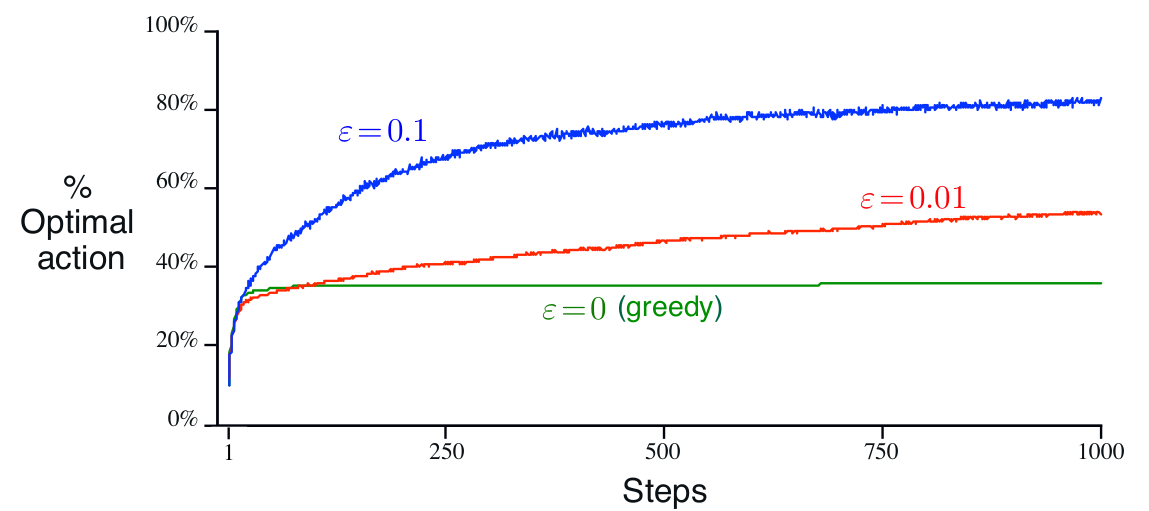
\includegraphics[scale=0.35]{images/eps_vs_optAction.png}
    \caption{Average performance of three agents using different $\epsilon$.  The data is averaged over 2000 runs.  Figure from \textit{Reinforcement Learning: An Introduction} by Sutton and Barto (2018).}
    \label{fig: eps_figure}
\end{figure}

During implementation, $\epsilon$ should decay out as $Q_t(u)$ approaches $q_*(u)$ to ensure knowledge of the agent is being adequately exploited. For non-stationary problems where the $Q$ values change, $\epsilon$ must be greater than 0 for all $t$ to ensure continued exploration.

Algorithms to solve the \textit{k}-armed bandit problem are easily applied to situations where the concept of state is inert and only the actions are of concern;  a near impossibility in the real world.  

\subsubsection{Contextual Bandit}

A natural extension of the \textit{k}-armed bandit is associative search.  In associative search (sometimes called contextual bandit), different policies are associated with different situations \cite{bartosuttonbrouwer}.  Equation \ref{eq: state-action-value} is the extension of Equation \ref{eq:01value} in the associative search problem.

\begin{equation}
    \centering
    q_*(x, u) = \mathbb{E}[R_t | X_t = x, U_t = u]
    \label{eq: state-action-value}
\end{equation}

Associative search is known as the method between \textit{k}-armed bandits and reinforcement learning.  In associative search, the objective is to associate optimal policies to different situations, but only maximizing the \textit{immediate} reward.  Often times, near term sacrifices are required to initiate the trajectory to a large lump sum reward at the terminal state.  For example, heavy capital and time investment is required for University in the short term.  However, the long term gain is so great that it outweighs the short term losses, making going to University an optimal policy for many individuals.

In order to find the true optimal policy (i.e., policy that returns the greatest rewards over a long time period), the topic of reinforcement learning is developed.  In reinforcement learning, sequential decision making is explored to identify the delayed reward signals from different actions and to ultimately find the optimal policy, $\pi^*$.  

% %%%%%%%%%%%%%%%%%%%%%%%%%%%%%%%%%%%%%%%%%%%%%%%%%%%%%%%%%%%%%%%%%%%%%%%%%%%%%%%%%%%%%
% % MARKOV DECISION PROCESSES
% %%%%%%%%%%%%%%%%%%%%%%%%%%%%%%%%%%%%%%%%%%%%%%%%%%%%%%%%%%%%%%%%%%%%%%%%%%%%%%%%%%%%%

% %%%%%%%%%%%%%%%%%%%%%%%%%%%%%%%%%%%%%%%%%%%%%%%%%%%%%%%%%%%%%%%%%%%%%%%%%%%%%%%%%%%%%
% MARKOV DECISION PROCESSES
%
% Introduction to MDPs, finite MDPs, infinite MDPs
% Semi MDPs
% Partially Observable MDPs
%
%%%%%%%%%%%%%%%%%%%%%%%%%%%%%%%%%%%%%%%%%%%%%%%%%%%%%%%%%%%%%%%%%%%%%%%%%%%%%%%%%%%%%

\section{Markov Decision Processes}
In the face of uncertainty, the agent's \textit{sequential} decision making is formalized in the Markov decision process (MDP). The general MDP framework is shown in Figure \ref{fig:01mdp} and contains two components: the \textbf{agent} and the \textbf{system}. The \textbf{agent} is a continuously learning decision maker and is mathematically represented by the RL algorithm. Objectively, the agent will undergo numerous meaningful interactions with the system to ultimately learn the optimal policy, $\pi^*$ (i.e., the optimal decisions given different situations). Conversely, the \textbf{system} contains all elements the agent cannot arbitrarily control. In process control, the ambient temperature, actuators, and even the wires transporting the control signals are all part of the system because the agent cannot \textit{deterministically} manipulate them. 

\begin{figure}[H]
    \centering
    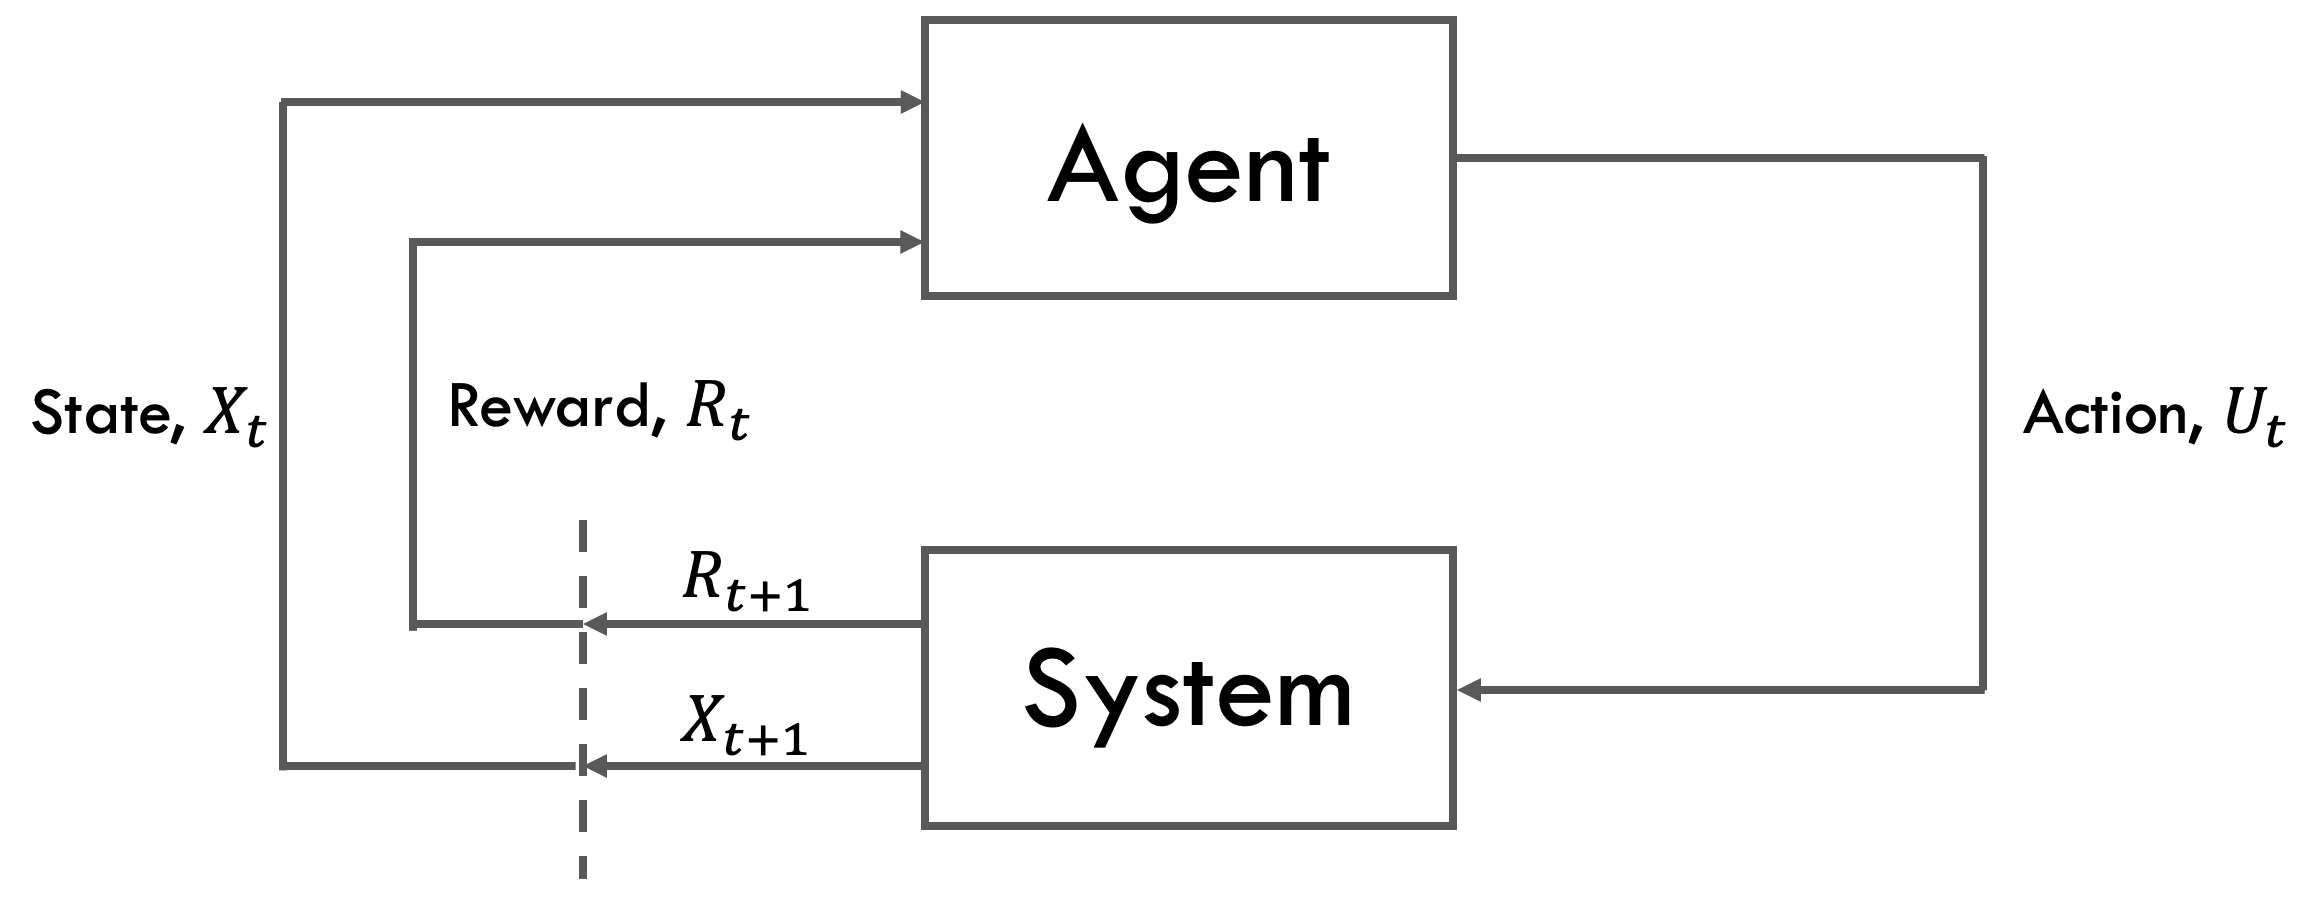
\includegraphics[width=0.56\textwidth]{images/ch1/MDP.jpeg}
    \caption{The general Markov decision process framework. Original image from \cite{sutton}.}
    \label{fig:01mdp}
\end{figure}   

Mathematically, the MDP is a discrete representation of the stochastic optimal problem and a classical formulation of \textit{sequential} decision making where both the immediate and long term consequences are explicitly considered \cite{bellman1, mdp_bellman}. Many definitions of the MDP exist and are equivalent up to small alterations of the process.  One comprehensive definition is that a MDP is a tuple $\mathcal{M}$, is a tuple $(\mathcal{X}, \mathcal{U}$, $P(x', r|x, u), \gamma, R)$ comprised of the following\cite{ng_ref12}:
\begin{itemize}
    \item $x \in \mathcal{X}$: \textbf{State} space of the system at each time step. Common states in industrial processes include temperatures, valve positions, pressures, flow rates, etc.
    \item $u \in \mathcal{U}$: Bounded \textbf{action} space of the agent, ($\mathcal{U}$ $ \geq 2 $). In traditional control, this is the \textbf{bounded input signals} sent to the actuators.
    \item $R \in \mathbb{R}$: Expected \textbf{reward} signal after performing action $u$ in state $x$. Reward functions are designed based on a desired performance metric.  In control theory, the reward function is known as the \textbf{objective function}.  Typically, $|R| \leq \mathcal{R}$ for convergence guarantees.
    \item $p(x', r|x, u)$: Systems \textbf{dynamics function}. Formally, it is the probability of transitioning to $x'$ and receiving $r$,  given states $x \in \mathcal{X}$ and performing action $u \in \mathcal{U}$. Mathematically, it is described by the following:
    \begin{equation}
        p(x', r | x, u) \dot{=} Pr\{X_t = x', R_t = r | X_{t - 1} = x, U_{t-1} = u\}
        \label{eq:transition_prob}
    \end{equation}
    where $p$ describes the system \textbf{dynamics} and $Pr$ denotes the probability operation \cite{sutton}. Additionally, $p$ satisfies the following equality:
    \begin{equation}
        \sum\limits_{x' \in \mathcal{X}} \sum\limits_{r \in \mathcal{R}} p(x', r | x, u) = 1, \forall x \in \mathcal{X}, u \in \mathcal{U}
        \label{eq:prob}
    \end{equation}
    Notice here that $p$ is only a function of the \textit{immediate past}, thus assuming that $x_{t - 1}$ and $u_{t-1}$ captures the complete history. This is known as the Markov property and its underlining assumptions are critical for successful process control applications using RL. Additionally, note that when the state and actions are formulated as augmented past information: $x_{t-1} = [s_{t-1}, s_{t-2}, ... s_{t-N}], u_{t-1} = [a_{t-1}, a_{t-2}, ..., a_{t-N}]$, where $s_{t-N}$ and $a_{t-N}$ denotes the past states and actions, the system is still Markov because decisions can be made exclusively using $x_{t-1}$ and $u_{t-1}$. 
    \item $\gamma$: \textbf{Discount factor} associated with uncertainty of the future, ($0 \leq \gamma \leq 1)$. $\gamma < 1$ is also a requirement for continuous processes to guarantee eventual convergence.
\end{itemize}

There exists three different MDPs: fully observable MDP (FOMDP), partially observable MDP (POMDP), and semi MDP (SMDP). Table \ref{tab:01mdps} shows a general guideline on the different MDPs.

\begin{table}[H]
\caption{A comparison of different Markov decision processes.}
\centering
\begin{tabular}{c|c|c}
\textbf{FO-MDPs}	& \textbf{S-MDPs}	& \textbf{PO-MDPs}\\
\hline
All states observable		  & All states observable			& Some states observable \\
Discrete time		          & Continuous time	             	& Discrete time \\
\end{tabular}
\label{tab:01mdps}
\end{table}

\subsection{Fully Observable Markov Decision Processes}
Fully observable Markov decision processes are the simplest and serves as the foundational framework.  They are mainly applied to discrete systems with fixed sampling times where transition dynamics are unimportant and all states are observable (measurable in control literature). Here, the agent starts in some initial states, $x_0$. At each time $t$, the agent maps $x_t$ to some $u_t$ corresponding to its policy, $\pi_t$.  Given $x_t$ and $u_t$, the system will then transition to some new states $x_{t+1}$ dictated by Equation \ref{eq:transition_prob} while outputting reward signal $R_{t+1}$ based on the reward function. In regulation and set-point tracking problems, this reward function is typically the squared tracking error between $x_t$ and $x_{sp}$.  By repeating this cycle many times, the agent is able to traverse through some sequence, $x_t, u_t, R_{t+1}, x_{t+1}, u_{t+1}, R_{t+2}, x_{t+3}, ...$ and accumulate \cite{sutton}:
\begin{align}
G_t &= R_{t+1} + \gamma R_{t+2} + \gamma^2 R_{t+3} ... \\
    &= \sum\limits^{\infty}_{k = 0} \gamma^k R_{t+k+1}
\label{eq:return}
\end{align}
where $G_t$ denotes the cumulative discounted return at time $t$ and $\gamma$ is the discount factor to capture the future uncertainty. MDPs can represent both finite or infinite systems; the former describes episodic tasks with explicit terminal states while the latter describes tasks that continue forever.  Intuitively, most two-player board games such as Checkers, Chess, or Go are finite MDPs where the game is terminated after one player is defeated.  Contrarily, an infinite MDP system could be the control system in an industrial process. For infinite MDP systems, $\gamma < 1$ is a necessary condition to keep $G_t$ bounded. Ultimately, the agent is tasked with finding the optimal policy, $\pi^*$, that maximize $G_t$, and subsequently the value function, over $N$ steps. The value function for each state is given as \cite{sutton}:
\begin{align}
    v_\pi (x) &\dot{=} \mathbb{E}_\pi [G_t | X_t = x] \\
              &= \mathbb{E}_\pi \left[\sum\limits^\infty_{k=0} \gamma^k R_{t+k+1} | X_t = x \right] \\
              &= \mathbb{E}_\pi [R_{t+1} + \gamma G_{t+1} | X_t = x]
    \label{eq:value_func}
\end{align}
where $v_\pi (x)$ is the value function of $x$ under policy $\pi$. Theoretically, the existence and uniqueness of $v_{\pi}$ is guaranteed for continuous systems where $\gamma < 1$ or in systems with guaranteed termination.  Compared to Equation \ref{eq:01value}, Equation \ref{eq:value_func} takes the expectation of $G_t$; therefore, explicitly optimizing the long term returns rather than only the immediate rewards. The action-value formulation of Equation \ref{eq:value_func} is:
\begin{align}
    q_\pi (x, u) \; &\dot{=} \; \mathbb{E}_\pi [G_t | X_t = x, U_t = u] \\
                 &= \mathbb{E}_\pi \left[\sum\limits^\infty_{k=0} \gamma^k R_{t+k+1} | X_t = x, U_t = u \right], \forall x, u \in \mathcal{X, U}
    \label{eq:a_value_func}
\end{align}
FOMDPs work well for discrete systems where all states are observable.  However, system states in industrial processes are often unobservable (unmeasurable in control) due to limited hardware or engineering limitations. In such systems, the Markov property no longer holds resulting in sub-optimal decision making of the agent.





\subsection{Partially Observable Markov Decision Processes}
Partially observable Markov decision processes (POMDPs) extend upon the concepts of FOMDPs and represent systems with unobservable states. In RL literature, observability is equivalent to measurability in control; thus, the two terms are used interchangeably here-forth. In FOMDPs, the current state $x_t$ at each time $t$ is fully observable. In the more general setting of POMDPs, the entire state vector describing the agent's current situation is no longer available. Instead, the agent only has access to a set of possible observations $\mathcal{O}$. At each time $t$, the agent sees observation $o_t$ which correspond to probability distributions over states.  Using $o_t$, the agent can infer the states it \textit{might} currently be in \cite{ng_ref12}. Relating to a process control setting, existing sensors typically only measure a subset of the current states; however, by using available measurements, one can infer the remaining unmeasurable states using probabilistic approaches.

Generally, finding $\pi^*$ in a POMDP setting is significantly harder compared to FOMDPs.  Even finding a near-optimal policy is at least NP-hard (non-deterministic polynomial time) \cite{pomdp_time}.  Furthermore, even agents with access to all the system's true value functions are unable to behave optimally in a POMDP setting because the current states are unknown \cite{ng_ref12}. 

Belief states is one method for agents to behave optimally in POMDPs. On a high level, belief states transform the POMDP setting into its FOMDP counterpart through a probabilistic approach. Specifically, belief states, $b$, are probability distributions over states deduced using previous observations and actions. The probability distributions represent what the agent thinks its current state is. Using these probabilities, the agent can compute scalar value functions of each state-action pair and use these to act "optimally".  Note here that the agent's behaviour is optimal given the available information, and not optimal with respect to the system. An quantitative example is provided below:
\begin{quote}
    Suppose an agent exists in a two-input two-output (TITO) POMDP setting with two unobservable states ($x_1$ and $x_2$) and two actions ($u_1$ and $u_2$) and suppose the problem is only concerned with the immediate consequences (for longer horizons, the agent must also consider the long term rewards, making the example less intuitive). In this system, there are four value functions, one for each state-action pair. Suppose $u_1$ earns a reward of 2 in $x_1$ and 0 in $x_2$.  Similarily, $u_2$ earns a reward of 0 in $x_1$ and 1 in $x_2$.  Given $b_t = [0.2, 0.8]$ (probabilities of being in $x_1$ and $x_2$, respectively), then $Q(b_t, u_1) = 0.2 \cdot 2 + 0.8 \cdot 0 = 0.4$ and $Q(b_t, u_2) = 0.2 \cdot 0 + 0.8 \cdot 1 = 0.8$, resulting in $u_2$ being the optimal action.
\end{quote}

In control theory, observers, such as soft sensors, are used to estimate unmeasurable states.  Observers are typically $1^{st}$ principles, data driven, or probabilistic models. The concept of belief states is very similar to observer design in control theory. Traditionally, Kalman filter is a widely used observer design. Conversely, recurrent neural networks (RNNs) are widely used for belief state estimation in RL. The performance of RNN was compared with Kalman filter in \cite{RNNvsKF}, drawing similarities of the two methods' objective, theory, and performance.

System representations using FOMDPs and POMDPs work well in discrete tasks where transition times are constant and transition dynamics are disregarded; however, both topics are paramount for continuous optimal control.  







\subsection{Semi Markov Decision Processes}
Semi-Markov decision processes (SMDP) extend the concepts of MDPs to continuous time and can represent unknown transition times and system dynamics. In SMDPs, the transition dynamics of the system are explicitly captured using reward function \cite{continuous_rl_ref14}:
\begin{equation}
R(x_t, x_{t+1}, u_t) = \int\limits^\infty_0 \int\limits^t_0 e^{-\beta s} \rho(x_t, \pi (x_t))dsdF_{x_t, x_{t+1}}(t | \pi (x_t))
\label{eq:reward_rate}    
\end{equation}
where $R(x_t, x_{t+1}, u_t)$ is the reward when transitioning from $x_t$ to $x_{t+1}$ after performing action $u_t$, adjusted for the unknown transition time. Here, $\rho(x_t, \pi(x_t))$ represents the mean reward during the transition following policy, $\pi$. To obtain $\rho$, intermediate rewards are calculated at each time step in the transition period to explicitly capture transition information. $F_{x, x_{t+1}}(t, u)$ denotes the probability distribution of the transition time from $x_t$ to $x_{t+1}$.  Finally, $\beta > 0$ is the \textit{constant} discount factor in SMDPs. High $\beta$ results in short-sighted agents. In SMDPs, the transition time is no longer constant.  Thus, the discount factor is corrected for transition time during each update step.  The corrected discount factor is:
\begin{equation}
    \gamma(x_t, x_{t+1}, u) = \int\limits^{\infty}_0 e^{-\beta t} dF_{x_t, x_{t+1}}(t | \pi_t)
\end{equation}
where $\gamma (x_t, x_{t+1}, u_t)$ is the transition time adjusted discount factor. The value function for SMDPs is obtained through combining Equations \ref{eq:reward_rate} and \ref{eq:value_func}:
\begin{equation}
v_{\pi}(x_t) = \frac{1 - e^{-\beta \tau}}{\beta} R(x_t, x_{t+1}, \pi(x_t)) + e^{-\beta \tau}v_{\pi}(x_{t+1})
\end{equation}
where $\tau$ denotes the unknown transition time. The action-value variant is given by:
\begin{equation}
    q_{\pi}(x_t, u_t) = \frac{1 - e^{-\beta \tau}}{\beta} R(x_t, x_{t+1}, \pi(x_t)) + e^{-\beta \tau}  q_{\pi}(x_{t+1}, u_{t+1})
\end{equation}
By representing control environments as SMDPs, policies resulting in large overshoot, inverse response, or other undesirable dynamics will be minimized. Additionally, SMDPs can handle unknown transition times.  An intuitive example of SMDPs in process control is as follows:

\begin{quote}
Suppose a CSTR in a refinery must maintain a temperature of 200$^{\circ}$ C.  The temperature is regulated using cooling water via a heat exchanger.  A RL agent was tasked with maintaining the temperature set point. Suppose the CSTR is initiated at 220$^{\circ}$ C.  Agents using FOMDP representations may be overly aggressive and send large control actions because the reward is calculated \textit{right before} the next evaluation step. Therefore, input signals resulting in large overshoot or inverse response may be missed during the reward calculation. Contrarily, SMDPs consider the average reward accumulated throughout the transition to provide feedback to the agent, allowing the undesirable dynamics to be captured. Furthermore, the sampling time of SMDPs are not fixed (traditional representations evaluate after a set time period), enabling re-evaluation during the transitional period if unexpected events occur. In such scenarios, the discount factor will also be adjusted in accordance to the elapsed time from last evaluation.
\end{quote}









\subsection{Optimal Solution of the MDP}
The optimal solution to the RL problem refers to identifying a policy that generates the highest long term returns. Such a policy may not be unique; there may exist many optimal policies, where $v_{\pi^*_1} = v_{\pi^*_2} = ... = v_{\pi^*_N}$.  Formally, the optimal policy must satisfy the \textbf{principle of optimality}: the optimal policy $\pi^*$ is optimal if and only if $v_{\pi^*}(x) \geq v_{\pi \neq \pi^*}(x)$ for all $x \in \mathcal{X}$ \cite{PO}. Mathematically, the optimal value function is:
\begin{equation}
    v^*(x) \dot{=} \argmax_{\pi} v_{\pi}(x), \forall x \in \mathcal{X}
\end{equation}
with its action-value variant being:
\begin{equation}
    q^*(x, u) \dot{=} \argmax_{\pi} q_{\pi}(x, u), \forall x, u \in \mathcal{X, U}
\end{equation}
In a more explicit form, the optimal value function and action-value function written in terms of Equations \ref{eq:value_func} and \ref{eq:a_value_func} are given, respectively, by \cite{sutton}:
\begin{equation}
    v^*(x) = \argmax_{u} \mathbb{E}[R_{t+1} + \gamma v^*(X_{t+1}) | X_t = x, U_t = u]
    \label{eq:01valuefunc}
\end{equation}
\begin{equation}
    q^*(x, u) = \mathbb{E}\left[R_{t+1} + \gamma \argmax_{u_{t+1}} q^*(X_{t+1}, u_{t+1}) | X_t = x, U_t = u \right]
\end{equation}
Here, the $max$ operation denotes that the optimal action will be taken for the remaining of the trajectory. Theoretically, all optimal value functions can be explicitly solved using Equation \ref{eq:01valuefunc}; however, such a task would require unreasonable amounts of computation power for even simple systems. In the following section, three popular methods will be introduced to estimate the value and action-value functions in reinforcement learning.


% %%%%%%%%%%%%%%%%%%%%%%%%%%%%%%%%%%%%%%%%%%%%%%%%%%%%%%%%%%%%%%%%%%%%%%%%%%%%%%%%%%%%%
% % Reinforcement Learning
% %%%%%%%%%%%%%%%%%%%%%%%%%%%%%%%%%%%%%%%%%%%%%%%%%%%%%%%%%%%%%%%%%%%%%%%%%%%%%%%%%%%

% %%%%%%%%%%%%%%%%%%%%%%%%%%%%%%%%%%%%%%%%%%%%%%%%%%%%%%%%%%%%%%%%%%%%%%%%%%%%%%%%%%%%%
% Reinforcement Learning
%
% Introduction to MDPs, finite MDPs, infinite MDPs
% Semi MDPs
% Partially Observable MDPs
%
%%%%%%%%%%%%%%%%%%%%%%%%%%%%%%%%%%%%%%%%%%%%%%%%%%%%%%%%%%%%%%%%%%%%%%%%%%%%%%%%%%%

\section{The Reinforcement Learning Problem}

In general terms, reinforcement learning in an industrial setting is simply an agent undergoing meaningful interactions with the process to learn an optimal operating policy.  For added intuition, Figure \ref{fig: simple_rl} shows the information flow of an agent in process control. First, the agent observes some states, $x_t \in \mathcal{X}$, from the environment (some states may be unobservable).  Given $x_t$, the agent performs some controls actions, $u_t \in \mathcal{U}$ and receives a scalar reward signal, $r_{t+1} \in \mathcal{R}$.  Finally, the process will transition to some new states, $x_{t+1}$, given probability $P(x_{t+1}, r_{t+1} | x, u)$.

\begin{figure}[H]
    \centering
    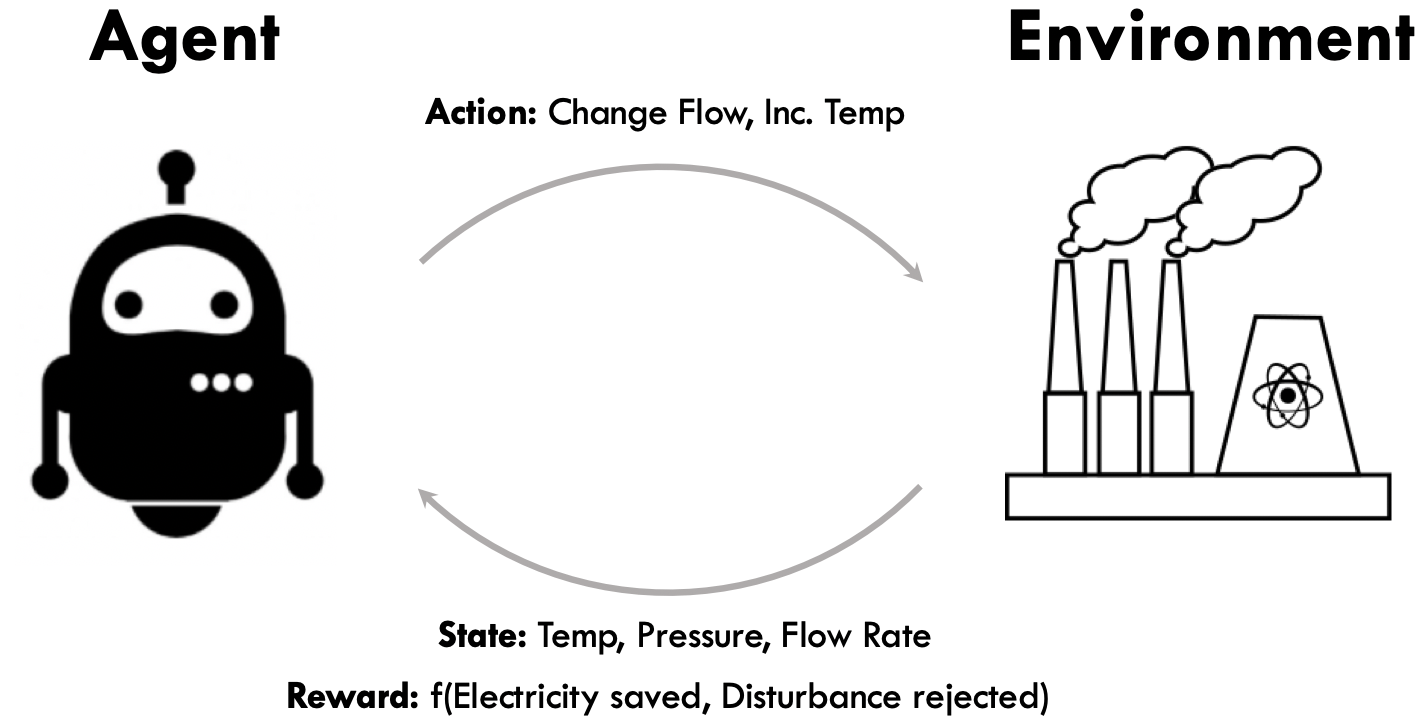
\includegraphics[scale=0.5]{images/ch1/RL.png}
    \caption{Basic setup of reinforcement learning where an agent interacts with the system.}
    \label{fig: simple_rl}
\end{figure}

The three main branches of reinforcement learning solutions are shown in Figure \ref{fig:RL_methods}. Starting from the left, dynamic programming (DP) methods can identify the exact value functions, but require a \textit{perfect system model} and is extremely computationally expensive, even for trivial tasks.  Comparatively, both Monte Carlo (MC) and temporal difference (TD) methods are approximate DP methods.  As such, they are less computationally demanding.  Additionally, MC and TD methods do not assume the presence of a system model and identifies the value functions through interactions with the environment. MC methods find the value functions through averaging the returns generated over many sampled trajectories of states, actions, and rewards.  One drawback is the significant variance in the sampled trajectories. Consequently, this may lead to poor reproducability in highly noisy systems. TD methods combine the best characteristics of DP and MC methods into one unifying approach. Like MC methods, TD learn from sampled data.  Like DP methods, TD performs update steps after each step. However, TD methods typically exhibit large bias (especially during initial learning episodes) due to estimating values through previously estimated values (known as bootstrapping). The general details of each method will be shown throughout this section.  For a comprehensive introduction to each algorithm, see \cite{sutton}.

\begin{figure}[H]
    \centering
    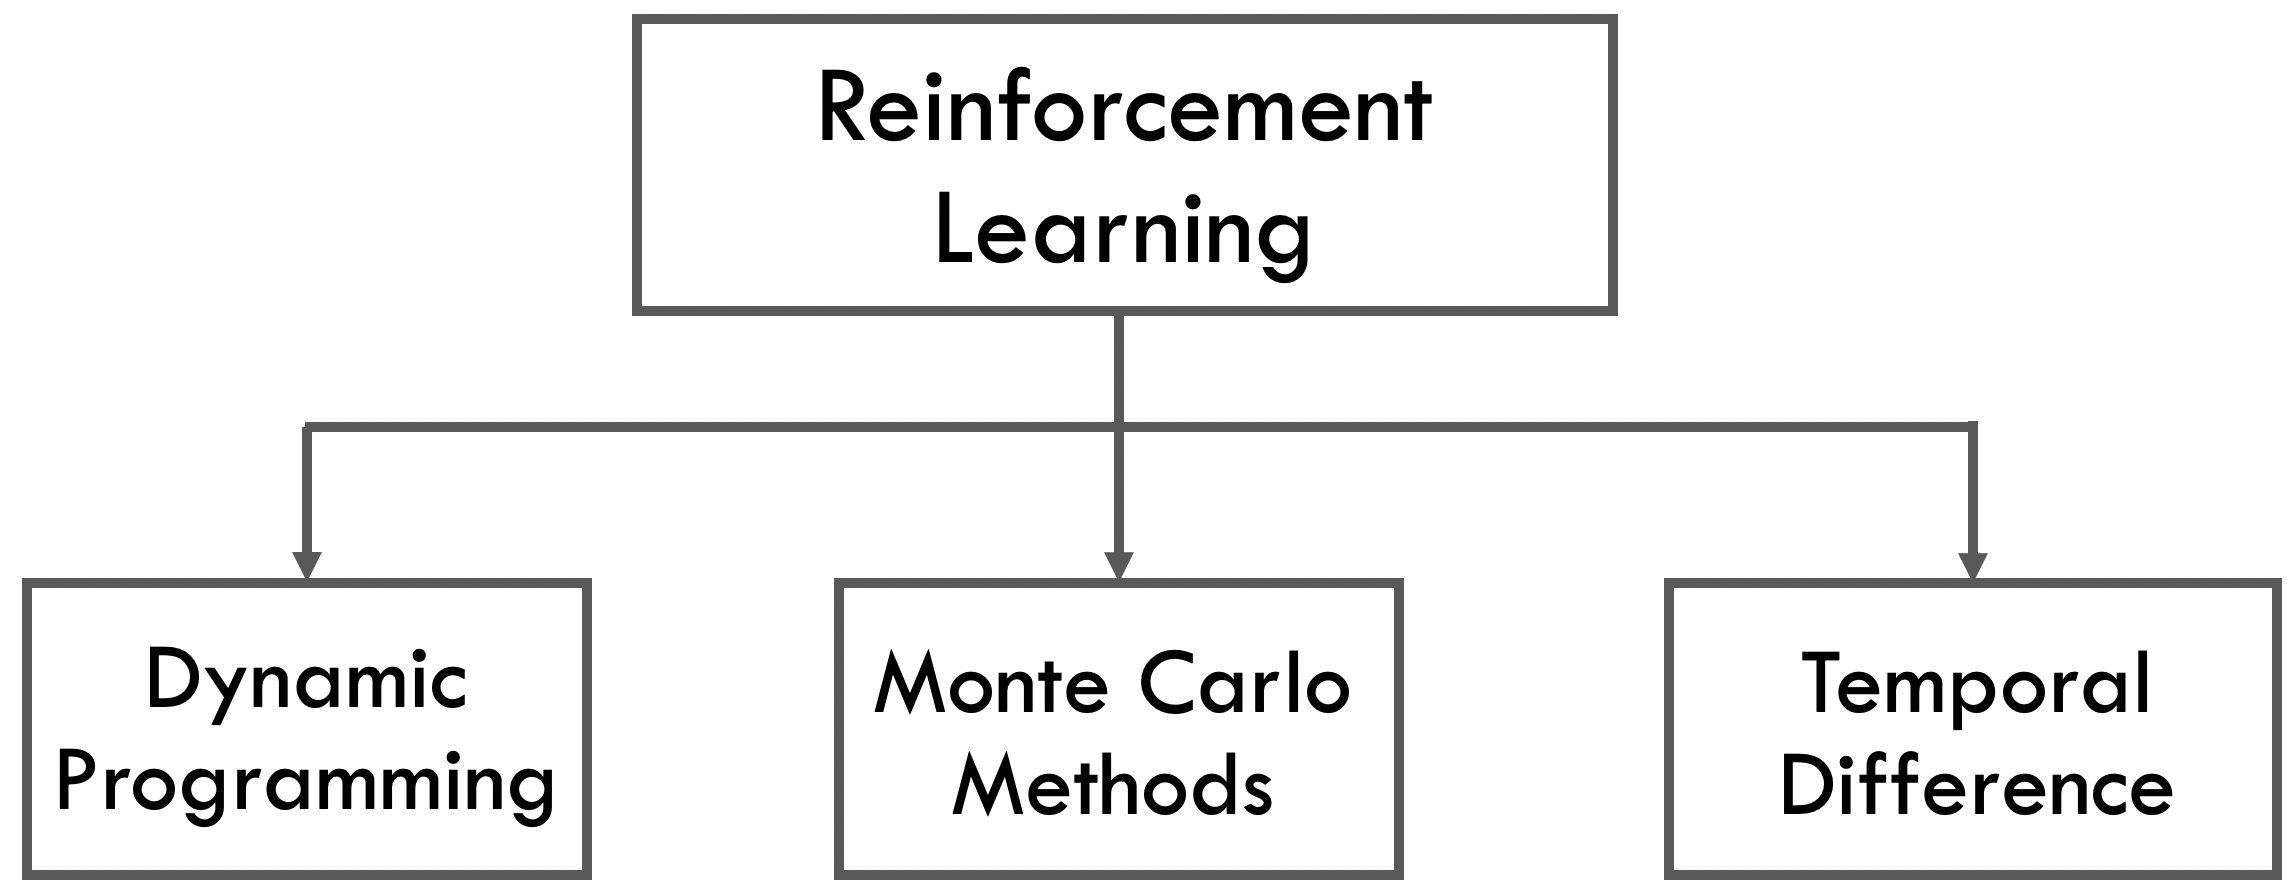
\includegraphics[width=0.6\textwidth]{images/ch1/RL_methods.jpeg}
    \caption{The sub-components of machine learning.}
    \label{fig:RL_methods}
\end{figure}   


\subsection{Dynamic Programming Methods}
Dynamic programming algorithms identify the exact value functions through an iterative procedure using the system dynamics function. In real life applications, DP algorithms are rarely used due to their unreasonable computational cost for even trivial problems. Nevertheless, the ideas of DP serve as the fundamentals for modern approaches. Policy iteration and value iteration are two common techniques in DP.  

As an overview, policy iteration searches for the optimal policy by iterating through infinitely many policies, $\pi \in \Pi$, storing only the policy corresponding to the highest cumulative returns.  The optimal policy is assumed to be found when $G_{\pi}$ can no longer be improved.  Policy iteration is comprised of two phases: policy evaluation and policy improvement. \textbf{Policy evaluation} computes the value functions and cumulative returns of the system under $\pi$ through an iterative approach. Value functions are initialized as 0, and are solved iteratively using:
\begin{equation}
    v_{k+1, \pi}(x) = \mathbb{E}_{\pi}[R_{t+1} + \gamma v_{k, \pi} (x_{k+1})]
\end{equation}
$$ v_0(x) = 0, \; \forall x \in \mathcal{X}$$
where $k$ denotes the $k^{th}$ update.  Here, $v_{k+1, \pi}(x)$ is the predicted value function for $x$ under policy $\pi$ after $k+1$ update steps.  As $k \rightarrow \infty$, $v_{k}(x) \rightarrow v_{\pi}(x)$ for all $x \in \mathcal{X}$ (i.e., the value functions converge to the true value functions under $\pi$). However, there often exists a $\pi'$ where $v_{\pi'}(x) \geq v_{\pi}$.  \textbf{Policy improvement} identifies such situations.  Once identified, current policy $\pi$ will violate the principle of optimality, hence deeming it ineligible for being the optimal policy. Then, the value functions of $\pi'$ will be identified in the next policy evaluation. This procedure will continue iteratively and infinitely until a policy where $v_{\pi^*}(x) \geq v_{\pi \neq \pi^*}(x)$ for all $x \in \mathcal{X}$ is found. After such a policy is identified, it is regarded as the optimal policy.

Figure \ref{fig:policy_iteration} shows a visualization of the policy iteration algorithm.  It can also be described using the following \cite{sutton}:
\begin{equation}
    \pi_0 \xrightarrow{\text{E}} 
    v_{\pi_0} \xrightarrow{\text{I}} 
    \pi_1 \xrightarrow{\text{E}}
    v_{\pi_1} \xrightarrow{\text{I}} 
    \pi_2 \xrightarrow{\text{E}} ... \xrightarrow{\text{I}} 
    \pi^* \xrightarrow{\text{E}}  v^*
\end{equation}
where $\xrightarrow{\text{E}}$ and $\xrightarrow{\text{I}}$ denotes the policy evaluation and policy improvement steps, respectively. From Figure \ref{fig:policy_iteration}, the agent starts with some arbitrary policy and performs policy evaluation. Initially, a large gap exists between $V_{\pi}$ and $\pi$.  As the iterative procedure proceeds, the gap is continuously reduced until $V_{\pi}, \pi \rightarrow V^*(x), \pi^*$. In industrial applications, the required iterative procedure for each policy evaluation is far too expensive for any non-trivial tasks.

\begin{figure}[H]
    \centering
    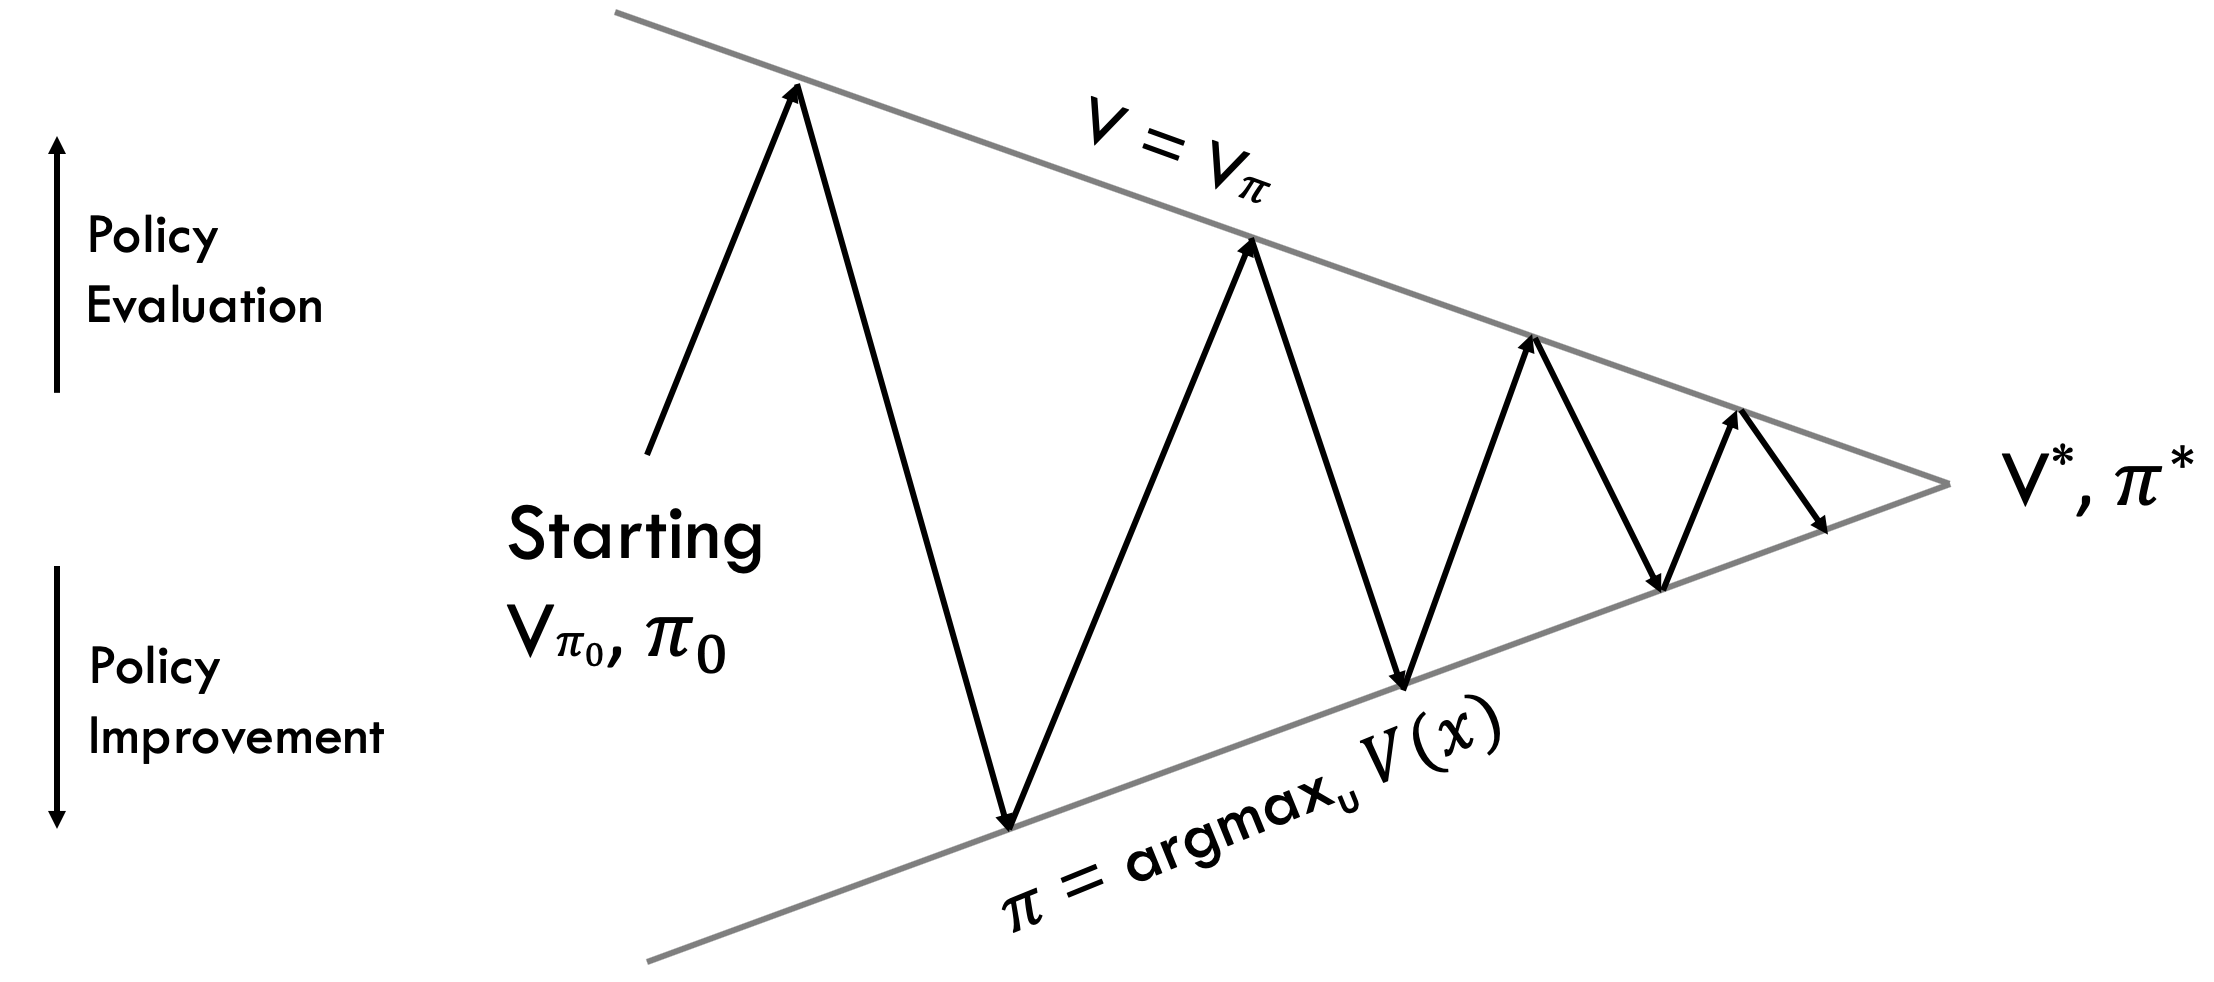
\includegraphics[width=0.68\textwidth]{images/ch1/policy_iteration.jpeg}
    \caption{A visualization of the policy iteration algorithm. Original image from \cite{silver_class}.}
    \label{fig:policy_iteration}
\end{figure}   

To improve upon these computational issues, value iteration was proposed.  Value iteration finds the optimal policy through identifying the optimal value functions instead. Intuitively, value iteration is a special case of policy iteration where the policy evaluation is terminated after one step.  From the value functions of each state, $\pi^*$ can be found by traversing through the states corresponding to the highest values. Note that the optimal policy can only be found using $V(x)$ if a dynamics equation of the system is provided. Without it, $Q(x, u)$ must be identified instead to behave optimally. The policy evaluation for the value iteration algorithm is given as:
\begin{equation}
    v_{k+1}(x) = \max_u \mathbb{E}[R_{t+1} + \gamma v_k(x_{t+1})]
\end{equation}
\begin{equation}
    q_{k+1}(x, u) = \mathbb{E}[R_{t+1} + \gamma \max_{u_{t+1}} q_k(x_{t+1}, u_{t+1})]
\end{equation}
Here, the $max$ operation ensures that each $v_k(x)$ is updated using only the maximizing action so the \textit{optimal} value function can be identified. After all $v^*(x)$ are identified, an agent can behave optimally starting in any state assuming the agent takes the maximizing action at each time. Note that both policy and value iteration are \textit{bootstrap} methods. Bootstrapping in RL increases data efficiency while capturing long-term trajectory information; however, the method also introduces unintended biased. 

In industry, both policy and value iteration have limited utility because their updates are far too computationally expensive. In high dimensional settings, even one iterative step may be intractable; therefore, even with value iteration's reduced computational complexity, it is still infeasible for most complex problems. Asynchronous dynamic programming methods further reduces computational complexity by only updating frequently visited states. However, agents are rendered hopeless in states that are rarely encountered. Although, such a methodology mimics human behaviour where encounters can be handled effectively and efficiently and more exotic situations may catch us by surprise. Nonetheless, such methods still require system models to be explicitly provided, an extremely rare case in industry.

\subsection{Monte Carlo Methods}
Monte Carlo methods no longer require explicit system models (a characteristic known as \textit{model-free}).  Instead, MC methods \textit{estimate} the average returns for different policies through sampling infinitely many sequences of states, actions, and rewards. As the samples increase, $v_k(x) \rightarrow v_{\pi}(x) \text{ for all } x \in \mathcal{X}$. Learning-wise, the average returns are updated at the end of each trajectory. Due to this, the finite tasks with explicit terminal states are typically solved using MC methods. For example, discrete manufacturing is an episodic task in process control. The system is reset after the assembly of each object (cars, toys, ...).  In episodic tasks, the value functions are updated naturally after each episode. However, most tasks in process control are continuous. Training a continuous agent using MC methods require additional modifications. One method is to pre-specify a length of time. After the time has elapsed, the agent will pause and update its value functions. 

Policy search in MC methods is similar to policy iteration. There exists three differences: 1) only visited states are updated; 2) updates use \textit{sampled} data instead of a model; 3) $q_{\pi}(x, u)$ is required and identified instead of $v_{\pi}(x)$. In MC methods, the action-value functions are identified because a model is not provided to the agent. Hence, the agent cannot behave optimally using only the value functions because the actions required to transition to the high value states are not known. Instead, action-values contain explicit information on the expected returns for each action in each state.  The iterative procedure of MC to compute the cumulative returns is given by: 
\begin{equation}
    \pi_0 \xrightarrow{\text{E}} 
    q_{\pi_0} \xrightarrow{\text{I}} 
    \pi_1 \xrightarrow{\text{E}}
    q_{\pi_1} \xrightarrow{\text{I}} 
    \pi_2 \xrightarrow{\text{E}} ... \xrightarrow{\text{I}} 
    \pi^* \xrightarrow{\text{E}}  q_{\pi_*}
\end{equation}
Intuitively, the agent is initiated in an unknown system and follows a certain policy, $\pi$, to traverse throughout the state space while collecting rewards after each decision. Eventually, the agent will reach a terminal state and conclude the episode. Upon termination, a sequence of returns $G_1, G_2, ..., G_{n - 1}$ can be generated using the received reward signals:
$$G_1 = R_{1} + \gamma R_{2} + \gamma^2 R_{3} + ... + \gamma^{n - 1}R_{n}$$
$$G_2 = R_{2} + \gamma R_{3} + \gamma^2 R_{4} + ... + \gamma^{n - 2}R_{n}$$
$$G_3 = R_{3} + \gamma R_{4} + \gamma^2 R_{5} + ... + \gamma^{n - 3}R_{n}$$
$$\vdots$$
$$G_{n - 1} = R_n$$
or:
\begin{equation}
    G_m = \sum\limits_{i=0}^n \gamma^{i} R_{m + i}
\end{equation}
where $G_m$ denotes the discounted cumulative return received on the $m^{th}$ step. Using $G_m$, the action-values can be computed for each step by:
\begin{equation}
    Q_{k+1}(x, u) = Q_{k}(x, u) + \frac{1}{k} \left[G - Q_k(x, u) \right]
    \label{eq:q_update_mc}
\end{equation}
where $Q_k(x, u)$ represents the $k^{th}$ action-value update and $G$ corresponds to the returns received after performing action $u$ in state $x$. Notice that as $k \rightarrow \infty$, $\frac{1}{k} \rightarrow 0$; therefore, this set-up is ineffective in non-stationary settings because the updates get infinitely small.  To extend Equation \ref{eq:q_update_mc} to non-stationary problems, $\frac{1}{k}$ is changed to a constant given by $\alpha$:
\begin{equation}
        Q_{k+1}(x, u) = Q_{k}(x, u) + \alpha \left[G - Q_k(x, u) \right]
        \label{eq:01mcupdate}
\end{equation}
where $\alpha \in (0, 1]$ is known as the learning rate (also called step size). The lower bound prevents $\alpha$ from approaching 0; therefore, allowing for continually adaptation in non-stationary problems. After each update of Equation \ref{eq:01mcupdate}, a new episode starts and the procedures are repeated.  As $k, \text{ \# of episodes } \rightarrow \infty, Q(x, u) \rightarrow q(x, u)$. Once $Q(x, u)$ converge, online action selection can be conducted by:
\begin{equation}
    \pi^*(x) = \argmax_{u} q(x, u)
    \label{eq:policy_extract}
\end{equation}
That is, $\pi^*$ is performing the greedy action in each state.  

\subsubsection{Exploration in MC}
Notice that bootstrapping is not used in MC methods.  In fact, all value functions are estimated independently. As such, MC methods do not suffer from bias issues; however, MC methods may suffer from large variances instead caused by the noise in each sampled trajectory \cite{sutton}. Moreover, exploration is mandatory in MC methods because the dynamics of the system are unknown to the agent. Through exploration, the agent can discover the dynamics of the system and the value functions for each state.  Typically, exploration in MC methods is conducted by initiating the agent in a random state at the beginning of each episode. After infinite episodes, all states will be visited infinitely many times.

MC methods allow the agent to learn solely from sampled data; however, the action-values are updated only after each episode. Such a procedure is unnatural in continuous systems (most systems in process control), disadvantageous long episode systems, and is not intuitive to human behaviour. For example, humans learn immediately after feedback, not in pre-set increments. Temporal difference methods combine the best features of DP and MC methods into one unifying algorithm.





\subsection{Temporal-Difference Methods}
Temporal difference (TD) methods are mathematically simple and cheap computationally compared to MC and DP methods. TD methods learn from experiences (like MC methods) and bootstraps (like DP methods). Furthermore, a dynamics model is not required in TD methods. Instead, the agent learns the dynamics from interactions. Moreover, TD methods update their value functions immediately after $x_{t+1}$ and $R_{t+1}$ are received. The TD update algorithm for value and action-value functions are given in Equations \ref{eq:td_value} and \ref{eq:td_action_value}, respectively \cite{td}:
\begin{equation}
    V(x_t) \leftarrow V(x_t) + \alpha \left[R_{t+1} + \gamma V(x_{t+1}) - V(x_t) \right]
    \label{eq:td_value}
\end{equation}
\begin{equation}
    Q(x_t, u_t) \leftarrow Q(x_t, u_t) + \alpha \left[R_{t+1} + \gamma Q(x_{t+1}, u_{t+1}) - Q(x_t, u_t) \right]
    \label{eq:td_action_value}
\end{equation}
where $\leftarrow$ is the update operator. At each update, the old value function is corrected as a function of the \textit{TD error} by a fixed amount determined by $\alpha$.  The TD errors are at each time $t$ is given as:
\begin{equation}
    \delta_t = R_{t+1} + \gamma V(x_{t+1}) - V(x_t)
    \label{eq:01td_error1}
\end{equation}
\begin{equation}
    \delta_t = R_{t+1} + \gamma Q(x_{t+1}, u_{t+1}) - Q(x_t, u_t)
    \label{eq:01td_error2}
\end{equation}
The first two terms, $R_{t+1} + \gamma V(x_{t+1})$, denote the predicted value function for $x$ in accordance with the last interaction.  $V(x_t)$ is the previously predicted value function for $x$. After infinitely many interactions with the system,  $V(x_t) \rightarrow v(x_t)$ (i.e., the estimated values converge to the true values). The action-values follow the same procedure. After convergence of the values and/or action-values, the optimal action selection is given in Equation \ref{eq:policy_extract}.

\subsubsection{Exploration in TD}
Like MC methods, TD methods are also \textit{model-free}; therefore, action-values are required for the agent to act optimally and exploration is mandatory. A simple and common exploration method used in TD methods is the $\epsilon$-greedy action selection. Here, the agent performs the greedy action with a $\epsilon \in [0, 1]$ probability of performing a random action. During training, $\epsilon$ is typically decayed throughout training.  At the beginning, $\epsilon$ starts at a high value because agent knows nothing. Eventually, $\epsilon$ decays to a low value when training is almost complete. 

Unfortunately, random exploration is sample inefficient and may require the agent to undergo thousands of interactions before learning anything meaningful. Learning can typically be significantly accelerated through a heuristics function $\mathcal{H}: \mathcal{X} \times \mathcal{U} \rightarrow \mathbb{R}$ \cite{harl}.  One such heuristics approach is the upper confidence bound (UCB) action selection algorithm \cite{ucb}. Here, exploration is promoted on states that have high potential to be optimal and is given by:
\begin{equation}
    U_t = \argmax_u [Q_t(x, u) + \mathcal{H}] 
    \label{ucb}
\end{equation}
The heuristics function here is given by:
\begin{equation}
    \mathcal{H} = c \sqrt{\frac{ln \; t}{N_t(x, u)}}
\end{equation}
where $c$ is the degree of exploration.  Large $c$ values promote greater degrees of exploration. Furthermore, $N_t$ is the number of times action $u$ was selected prior to time $t$. As $N_t(x, u) \rightarrow \infty$, the corresponding $Q(x, u)$ has been updated many times and becomes very accurate.  Hence, the heuristics function $\mathcal{H} \rightarrow 0$. 

\subsubsection{Popular TD Algorithms}
The two most popular TD algorithms are \textbf{SARSA} and \textbf{$Q$-learning}.  \textbf{SARSA} is an \textit{on-policy} algorithm. In such algorithms, the \textit{behaviour policy} and \textit{target policy} are identical.  Target policy refers to the goal policy of the agent.  Typically, this is the optimal policy.  Conversely, the behaviour policy, $b(u|s)$, is the policy used by the agent for decision making. In cases where the target and behaviour policy are identical, the agent is \textit{on-policy}. One flaw with \textit{on-policy} agents (assuming the target policy is the optimal policy) is that during training, the agent may quickly converge to a local optimum and never explore (since any policies containing exploration is not the optimal policy).  Ultimately, this results in a sub-optimal solution.  Contrarily, \textit{off-policy} agents, like \textbf{$Q$-learning}, typically follow exploratory policies during training to conduct deep exploration.  Then in online applications, the policy is swapped to the optimal policy. Moreover, \textit{off-policy} agents are \textit{guaranteed} to find the optimal policy assuming each state-action pair is visited infinite times and $b(u^* | s) > 0$ (i.e., probability of picking the optimal action under the behaviour policy is not 0) \cite{td}.

Since SARSA is \textit{on-policy}, the action-value function are updated using Equation \ref{eq:td_action_value} using the quintuple $(x_t, u_t, R_{t+1}, x_{t+1}, u_{t+1})$. $Q$-learning updates use only four parameters $(x_t, u_t, R_{t+1}, x_{t+1})$ through Equation \ref{eq:q_learning}:
\begin{equation}
    Q(x_t, u_t) \leftarrow Q(x_t, u_t) + \alpha \left[R_{t+1} + \gamma \argmax_{u_{t+1}} Q(x_{t+1}, u_{t+1}) - Q(x_t, u_t) \right]
    \label{eq:q_learning}
\end{equation}
In $Q$-learning, $u_{t+1}$ is not required because the action taken might follow a different policy compared to the target policy since the algorithm is \textit{off-policy}. Instead, Equation \ref{eq:q_learning} uses the $max$ operation to ensure $Q$-values are still updated towards the optimal policy. Ultimately, TD methods unify DP and MC methods, allowing the agent to learn from experiences and perform inter-episode updates to exploit the most recent learnings.

A detailed numerical example is provided in Chapter 4 where a tabular $Q$-learning algorithm was applied onto an industrial VFD system to conduct set-point tracking control.



\section{Summary of DP, MC, and TD}
The main features of DP, MC and TD methods are summarized in Table \ref{tab:dc_mc_td}. Overall, DP requires a dynamical model of the system to compute the value functions while both MC and TD methods can learn directly from interactions with the system. Both DP and TD methods use bootstrapping to estimate value functions; that is, they estimate the current value function based on previously estimated values. Bootstrapping is data efficient, but introduces large biases to the estimated values, especially in the early episodes.  Conversely, MC methods estimate the value functions of each state independently through sampling many system trajectories.  However, this method, instead, introduces high variance. For extremely noisy systems, the reproducability of the results may be low. Comparing the computational cost, DP methods require much more compared to MC or TD since all value functions are simultaneously solved. In MC methods, only the value functions that were visited in the sampled trajectories are updated.  Additionally, updates are conducted at the end of each episode and not after each step. Similar to DP methods, TD methods update the value function immediately after an experience; however, only the value function corresponding to the last visited state is updated. In terms of exploration, DP methods do not explore the system model (both transition probabilities and expected reward) is explicitly provided. MC methods explore by being initiated in a random state after each episode termination. In TD methods, agents explore by occasionally performing a random action.

\begin{table}[H]
\caption{A comparison of DP, MC, and TD methods.}
\label{tab:dc_mc_td}
\centering
{\scriptsize
\begin{tabular}{c|c|c|c}
 & \textbf{Dynamic Programming}	& \textbf{Monte Carlo} & \textbf{Temporal Difference}\\
\hline
Requires model	     	& Yes			& No     &  No \\
Estimate bias           & High			& Low    &  High \\
Estimate variance	    & Low			& High   &  Low \\
Computational cost		& High			& Medium &  Low \\
$v(x)$ update      	& All states simultaneously   & After a trajectory  &  After an experience \\
Exploration             & Not needed, all states update   & Random initialization  &  Performing a random action \\
\end{tabular}}
\end{table}




\section{Reward Design for Process Control}
The design of the reward function for process control applications is similar to MPC.  For regulation or set-point tracking problems, the MSE reward function can be used and is given by:
\begin{equation}
    r(x, u) = -(x_i - x_{sp})^2
\end{equation}
However, the agent may find it difficult to distinguish between small off-sets using this reward function.  For example, when the tracking error is 10, the reward is -100.  However, if the off-set is only 0.25 or 0.1, the agent would find it difficult to distinguish between the small rewards because the difference is miniscule compared to an error of 10.  To enhance this distinction, a Huber loss can be used \cite{huber}:
\begin{equation*}
    r(x, u) = \begin{cases}
    x_t - x_{sp} & \quad if \; |x_t - x_{sp}| > 1 \\
    (x_t - x_{sp})^2 & \quad otherwise
    \end{cases}
\end{equation*}
In this case, large errors are not squared, significantly reduce their magnitude.  In the tabular cases, this error works exceptionally well; however, not so much in deep RL.  Typically, the inputs to neural networks are normalized for sufficient learning \cite{NN}.  When normalizing the rewards, small errors will once again become indistinguishable.  In such a case, the following reward function typically works better:
\begin{equation*}
    r(x, u) = \begin{cases}
    x_t - x_{sp} & \quad if \; |x_t - x_{sp}| > 1, \\
    (x_t - x_{sp})^2 & \quad if \; 1 \geq |x_t - x_{sp}| > \eta, \\
    +1 & \quad otherwise
    \end{cases}
\end{equation*}
where $\eta$ is the maximum acceptable tracking error. Here, as the agent achieves states within $\eta$, the rewards are significantly increased.  Such an idea is similar to zone MPC, where the objective of the controller is to guide the trajectory within a zone \cite{zone_mpc}. Another flaw with deep RL comes from the noisy action signals.  For example, a normal human would not go and continuously change the air conditioning set-point if the temperature inside a house varies between $\ang{22.1}$ C to $\ang{22.2}$ C because the two temperatures are relatively the same.  In the case of deep RL, these are seen as two completely different states, and correspond to (slightly) different actions.  One could design a filter to remove such small actions from being sent to the system; however, adding a cost to the change in inputs is a more natural way to mitigate this:
\begin{equation}
    r(x, u) = -[(x_t - x_{sp})^2 + \nu \Delta u_t^2]
\end{equation}
where $\Delta u_t$ is the change in input in the last sampling time. The coefficient, $\nu$, is used to tune the effect of the action on the reward.  For example, if the system's input signals are typically small, a large $\nu$ would be used so the tracking error does not dominate the entire reward function.

In exotic scenarios where the optimal input is known, the reward function can become:
\begin{equation}
    r(x, u) = -[(x_i - x_{sp})^2 + (u_i + u_{ss})^2]
\end{equation}
Lastly, the rewards are sometimes clipped to avoid large TD errors causing numerical issues during bootstrapping \cite{reward_clip}.  From Equation \ref{eq:q_learning}, it can be seen that if $R(x, u) >>> Q(x, u), Q(x_{t+1}, u_{t+1})$, then the updated $Q(x, u)$ would be completely dominated by $R(x, u)$. Additionally, any future updates bootstrapping off $Q(x, u)$ would subsequently become dominated by its value. As such, rewards are clipped (bounded) within a range to prevent such issues. Unexpectedly large rewards may originate from incorrect sensor readings, which consequently leads to inaccurate reward signals being sent to the agent.  Reward clipping is conducted by:
\begin{equation}
    r(x, u) = min(max(r_t,\mu^- ), \mu^+)
    \label{reward_clipping}
\end{equation}
where $\mu^-$ and $\mu^+$ denotes the minimum and maximum rewards, respectively. 




\subsection{Reinforcement Learning vs. Other "Learnings"}

Reinforcement learning is a unique class of machine learning.  An ideal supervised learning model can only be as good as the subject matter expert providing the labels to the data set, which may not be 100\%.  For example, in a complex control task, the control law is usually highly non-linear. Control experts can try to provide control strategies for such systems, but optimality may not be guaranteed for highly non-linear systems. Also, supervised learning is used to generalize responses for occurrences not present in the data \cite{sutton}.  Reinforcement learning works by directly interacting with the environment \textit{without labels}. Through adequate exploration, reinforcement learning will identify peculiar features to optimally control such problems [citation required].  Reinforcement learning is \textit{similar} to unsupervised learning in terms of identifying hidden structures within the environment.  However, reinforcement learning tries to maximize an internal scalar reward signal, rather than purely data mining.

Evolutionary methods, a family of optimization algorithms such as genetic algorithm, are most similar to reinforcement learning.  For a control problem, such methods can apply multiple static policies for different operating regimes \cite{sutton}.  Policy search is conducted by first initiating $k$ random input trajectories of length $N$, generating input matrix $\mathbb{U}_{[k, N]} \in \pi$.  Subsequently, the loss, $J_U$, of each $U$ is calculated based on the objective function.  Input trajectories with the lowest loss move onto the next generation and generates new pseudo-random input trajectories.  This process is repeated until optimal policy, $\pi^*$ is found for each operating regime \cite{ga_for_control}.

Evolutionary methods work well when the policy space is sufficiently small, easy to find, or a lot of time is available for optimization.  The biggest advantage of such methods compared to reinforcement learning is that the whole state does not need to be known.  However, such methods does not capture the reinforcement learning fundamentals of mapping $X \rightarrow U$.  Unlike evolutionary methods, reinforcement learning keeps memory of each individual interaction making it a more data efficient approach \cite{sutton}.

%%%%%%%%%%%%%%%%%%%%%%%%%%%%% End Section Intro to RL %%%%%%%%%%%%%%%%%%%%%%%%%%%%%%%%%%%%%%%



%%%%%%%%%%%%%%%%%%%%%%% Begin Section Function Approximation %%%%%%%%%%%%%%%%%%%%%%%%%%%%%%%

\section{Function Approximation}
\subsection{Introduction to Function Approximations}
Prediction models have wide applications in all sectors of the economy.  To obtain the highest possible accuracy, one can simply have an infinitely large repository of previous examples.  When given any input, a suitable output can be generated by finding the exact solution in the repository.  For example, if the task is to predict the model of an automobile based on a picture and the dimensions of a car, one could obtain 100\% accuracy so long as every single car specification exists in a repository.  This idea sounds good in theory, but is only possible in real life if there exists infinite memory.  Function approximation aims to solve this problem by generating a model to generalize across a massively large repository of historical data.  Intuitively, the model stores the information at a much lower space complexity, for a cost of some reproduction error.  There is also a trade-off between the reduced space complexity and the reproduction error.  Large, complex models have increased space complexity but reduced error while small, simple models exhibit the opposite.  This section focuses on complex neural network models with high predictive capabilities.  In RL, function approximation is typically used to approximate the (action-) value functions or the policy itself.


\subsection{Neural Network Basics}
Neural networks are highly non-linear models that explore the individual and interaction effects of each variable with all other variables \cite{NN}. The general structure of a neural network is shown in Figure \ref{fig:08NN}.  Neural networks are comprised of an input layer, some hidden layer(s), and an output layer.  The input layer consists of the input data, while the hidden layer(s) and output layer consists of fitted weights and biases, $W_{n_x \times n_b}$ and $b_{n_b \times 1}$, respectively. Here, $n_b$ and $n_x$ denotes the batch size and the dimension of the input layer, respectively. In Figure \ref{fig:08NN}, $x_m$ denotes the $m^{th}$ input variable.  The superscript and subscript of $a$ denotes the hidden layer number and the node number in the corresponding layer, respectively.  Subscript $m_1$ to $m_r$ denotes the number of nodes in hidden layers 1 to $r$, respectively.  Finally, superscript $o$ denotes the output layer.
\begin{figure}[h]
    \centering
    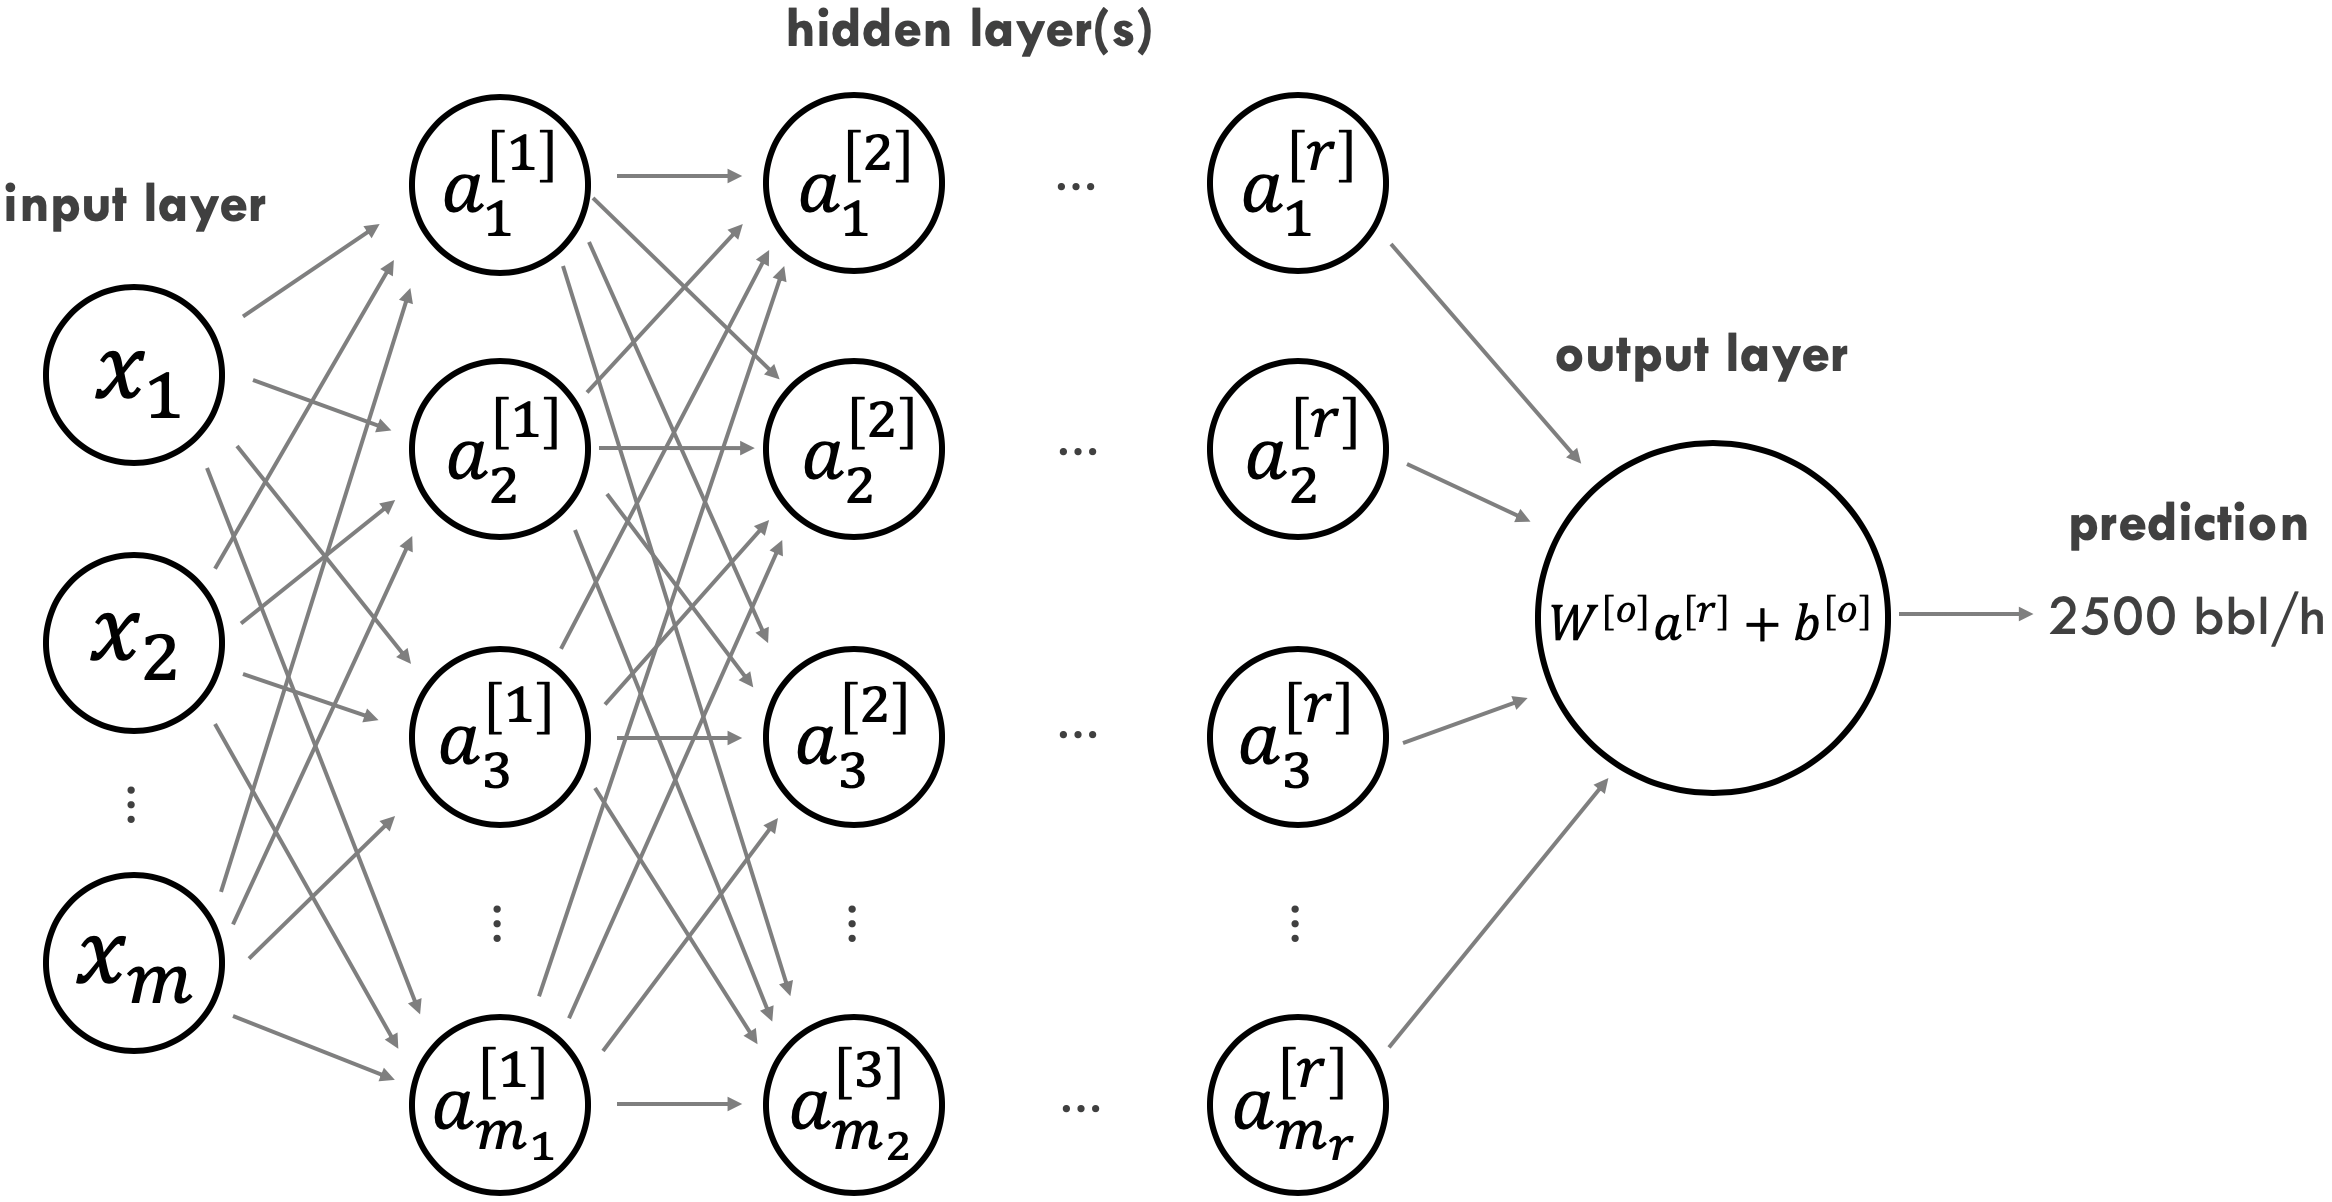
\includegraphics[width=0.9\textwidth]{images/ch1/08NN.png}
    \caption{Structure of a general neural network.}
    \label{fig:08NN}
\end{figure}


The details within a hidden layer's node is shown in Figure \ref{fig:08NNNode}. First, the outputs from the previous layer's nodes are inputted and multiplied by the weights of the current node.  The current node's bias is then added. If the current node is in the first layer, the outputs from the previous layer is replaced with the input variables. Afterwards, the output is sent to an action function to provide the non-linearity for any neural network model.  In this thesis, the rectified linear unit (ReLU) activation function is typically used and is given by:
\begin{equation}
    a^{[i]}_j=\begin{cases}
        y, & \text{if $y\geq0$}.\\
        0, & \text{otherwise}.
    \end{cases}
    \label{eq:08ReLU}
\end{equation}
where $i$ and $j$ denotes any hidden layer and any node number, respectively.  Two other popular activation functions are sigmoid and tanh given in Equations \ref{eq:01sigmoid} and \ref{eq:01tanh}, respectively.
\begin{equation}
    a^{[i]}_j = \frac{1}{1 + e^{-z}}
    \label{eq:01sigmoid}
\end{equation}
\begin{equation}
    a^{[i]}_j = \frac{e^z - e^{-z}}{e^z + e^{-z}}
    \label{eq:01tanh}
\end{equation}
where $e$ denotes the exponential operator and $z = Wx + b$. The sigmoid and tanh activation functions have lost popularity in recent years because they create the exploding/vanishing gradient effect.  This effect occurs because the derivatives of both the sigmoid and tanh functions are zero outside of a small section.  Additionally, the derivative at the inflection point is infinity.  Since neural networks are trained using backpropagation, often times, the gradient of the loss function becomes zero as it is backpropagated through the neural network during training.  Ultimately, this leads to significant difficulties in training neural networks (especially deep networks) \cite{vanish_grad}.  

\begin{figure}[h]
    \centering
    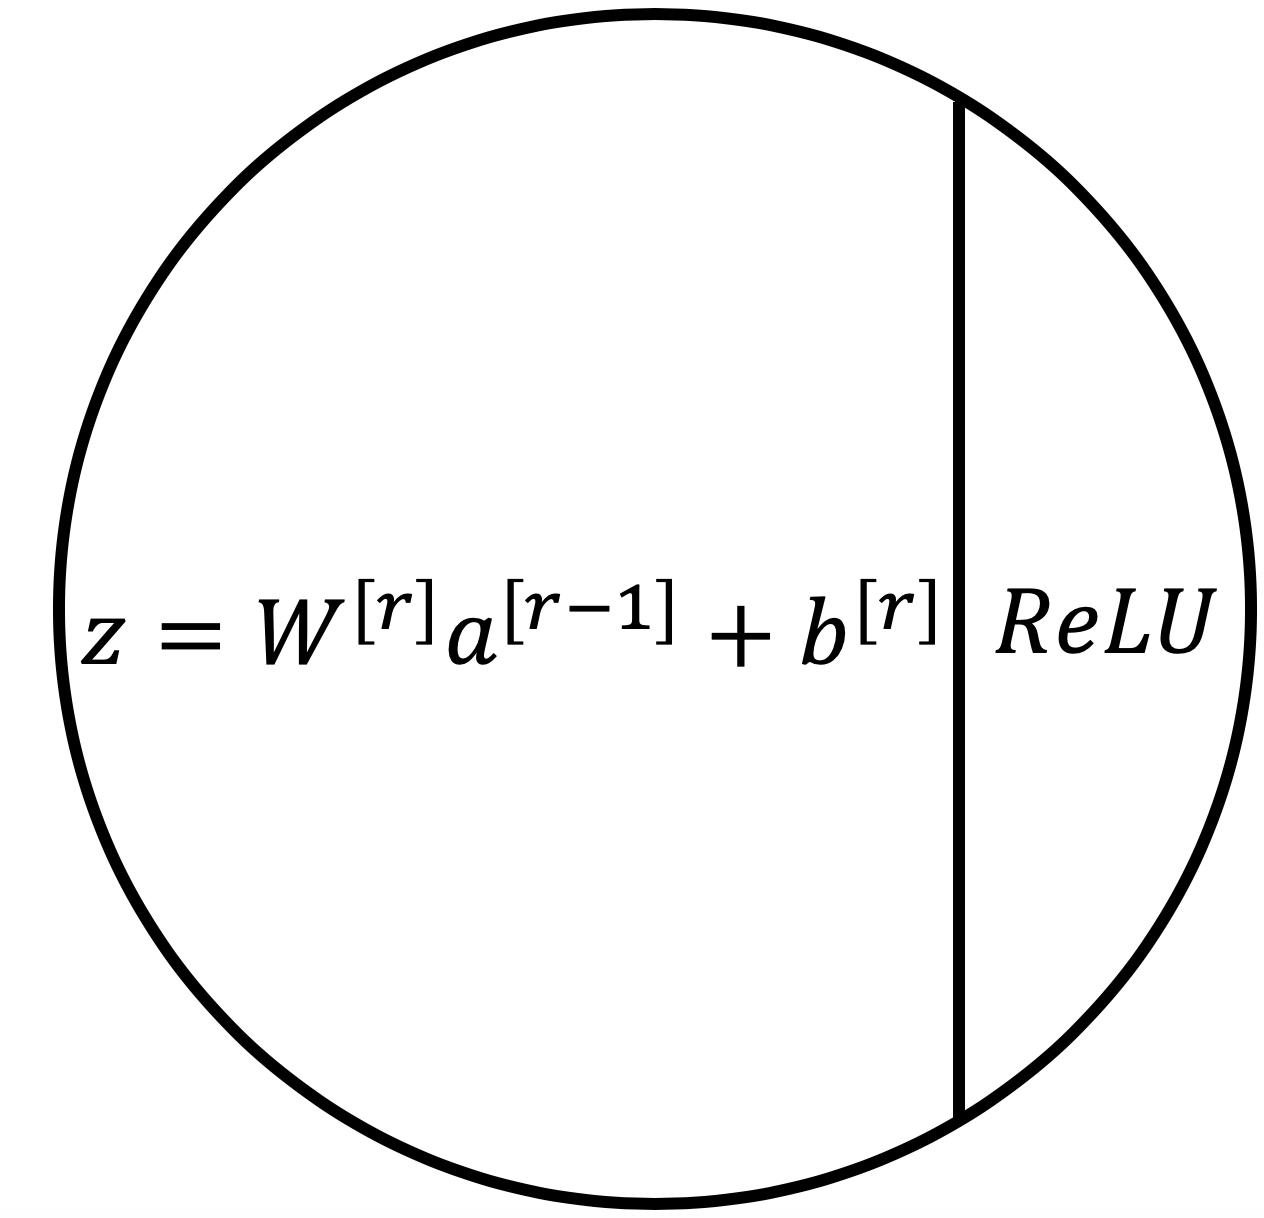
\includegraphics[width=0.3\textwidth]{images/ch1/08NNNode.png}
    \caption{Inside a hidden layer's node.}
    \label{fig:08NNNode}
\end{figure}

Mathematically, for one example with input vector $x$:
\begin{center}
    $z^{[1]}_j = W^{[1]}x + b^{[1]}$ \\
    $a^{[1]}_j = ReLU(z^{[1]}_j)$ \\
    $z^{[2]}_j = W^{[2]}a^{[1]}_j + b^{[2]}$ \\
    $a^{[2]}_j = ReLU(z^{[2]}_j)$ \\
    ... \\
    $z^{[r]}_j = W^{[r]}a^{[r - 1]}_j + b^{[r]}$ \\
    $a^{[r]}_j = ReLU(z^{[r]}_j)$ \\
    $y = W^{[o]}a^{[r]}_j + b^{[o]}$ \\  
\end{center}




\subsubsection{Neural Network Initialization}
Neural networks can be initiated in many ways. Although neural networks can be initiated as all zeros, such an approach is not symmetry-breaking resulting in all neurons performing the same calculations \cite{NN}.  Ultimately, this results in all neurons outputting the same values rendering the whole network useless.  Therefore, a primitive approach to overcome this was to initialize the neural network weights as random near-zero values. This method was symmetry-breaking, but such networks required long training times, especially in deep learning \cite{xavier_init}. In 2010, Xavier and Bengio published one of the first papers to explicitly study neural network initialization.

In \cite{xavier_init}, the the Xavier initializer was proposed to equalize the variance of the outputs of each layer with the variance of its inputs. More specifically, the biases of each layer was initialized as zero, but the weights were initialized as:
\begin{equation}
    W \thicksim U \left[-\frac{\sqrt{6}}{\sqrt{n_j + n_{j+1}}}, \frac{\sqrt{6}}{\sqrt{n_j + n_{j+1}}}  \right]
    \label{eq:01xavier}
\end{equation}
where $U[-a, a]$ represents an uniform distribution bounded between $(-a, a)$.  Here, $n_j$ and $n_{j+1}$ denotes the size of the previous and current layers. The derivation of Equation \ref{eq:01xavier} assumed linear actions. When tested using sigmoid activation functions, the Xavier initialized neural networks showed substantially faster convergence times. Unfortunately, sigmoid activation functions were considered obsolete as time went on due to the exploding/vanishing gradients problem \cite{vanish_grad}.  

By 2015, He et al. proposed a new initialization method specialized for ReLU activation functions, known as the He initializer \cite{he_init}. He extended upon previous work by assuming a ReLU activation function instead of a linear one and obtained the weight initialization function given by:
\begin{equation}
    W \thicksim \mathcal{N} \left(0, \frac{2}{n_j}  \right)
\end{equation}
where $\mathcal{N}$ denotes the Gaussian distribution and $\frac{2}{n_j}$ denotes its standard deviation.  Like in \cite{xavier_init}, the He initialization showed substantially faster convergence times for neural networks compared to previous methods when using the ReLU activation function.

The advantages of each initialization are summarized in Table \ref{tab:01nn_init}

\begin{table}[H]
\caption{Comparing different neural network initialization methods.}
\label{tab:01nn_init}
\centering
{\footnotesize
\begin{tabular}{c|c|c|c}
\textbf{Zero init.} & \textbf{Random init.}	& \textbf{Xavier init.} & \textbf{He init.}\\
\hline
Does not work	     	& Simple but slow			& Ideal for sigmoid activations &  Ideal for ReLU activations \\
\end{tabular}}
\end{table}




\subsection{Cost Function for Neural Networks}
MSE is the typical cost function for regression tasks and is given by \cite{NN}:
\begin{equation}
    J(\theta) = \frac{1}{n}\sum\limits^n_{i=1}(\hat{y}_i - y_i)^2
    \label{eq:08MSE}
\end{equation}
where $J$ represents the loss.  Here, $n$ denotes the number of samples in the current optimization step. $\hat{y}_i$ and $y_i$ are the $i^{th}$ predicted and actual labels, respectively. The MSE cost function is typically selected due to its convex nature \cite{deeplearning_course}.


\subsubsection{Gradient Descent}
Given the cost function, the model parameters are updated using gradient descent. The general gradient descent formulation is given by Equation \ref{eq:08GradientDescent}.  
\begin{equation}
    \theta_j^{m+1} \leftarrow \theta_j^{m} - \alpha \frac{\partial J}{\partial \theta_j}
    \label{eq:08GradientDescent}
\end{equation}
where $\theta_j$ denotes the $j^{th}$ parameter (parameter includes both weights and biases) of the model.  Here, $m$ represents the $m^{th}$ update of gradient descent and $\alpha$ is the learning rate. Unfortunately, gradient descent can optimize quite slowly, especially for neural networks where the solution is highly non-convex. There are many different enhanced gradient optimization methods such as momentum gradient descent, AdaGrad, RMSprop, etc; however, adaptive momentum gradient descent (ADAM) method will be used for the remainder of this thesis \cite{ADAM}. Mathematically, ADAM combines momentum gradient descent and RMSprop into one unifying algorithm. ADAM improves upon Equation \ref{eq:08GradientDescent} by computing an adaptive learning rate for each parameter \cite{ADAM}. To do so, the exponentially decaying average of the past gradients and squared gradients of the weights and biases are computed and stored using Equations \ref{eq:08momentW} to \ref{eq:08squared_momentb}.
\begin{equation}
    V_{dW} = \beta_1 V_{dW} + (1 - \beta_1)dW
    \label{eq:08momentW}
\end{equation}
\begin{equation}
    V_{db} = \beta_1 V_{db} + (1 - \beta_1)db
    \label{eq:08momentb}
\end{equation}
\begin{equation}
    S_{dW} = \beta_2 S_{dW} + (1 - \beta_2)dW^2
    \label{eq:08squared_momentW}
\end{equation}
\begin{equation}
    S_{db} = \beta_2 S_{db} + (1 - \beta_2)db^2
    \label{eq:08squared_momentb}
\end{equation}
where $V$ and $S$ are the estimates of the gradient and squared gradients, respectively.  $V$ and $S$ are typically initiated as zero vectors and are heavily biased towards zero at initial steps.  Hence, the biases (numerical bias, not the neural network parameter bias) for the initial terms are corrected using:
\begin{equation}
    V_{dW}^{corrected} = \frac{V_{dW}}{1 - \beta_1^t}
\end{equation}
\begin{equation}
    V_{db}^{corrected} = \frac{V_{db}}{1 - \beta_1^t}
\end{equation}
\begin{equation}
    S_{dW}^{corrected} = \frac{S_{dW}}{1 - \beta_2^t}
\end{equation}
\begin{equation}
    S_{db}^{corrected} = \frac{S_{db}}{1 - \beta_2^t}
\end{equation}
Combining the above equations, the weights and biases are updated by:
\begin{equation}
    W_j \leftarrow W_j - \alpha \frac{V_{dW}^{corrected}}{S_{dW}^{corrected} + \epsilon}
\end{equation}
\begin{equation}
    b \leftarrow b - \alpha \frac{V_{db}^{corrected}}{S_{db}^{corrected} + \epsilon}
\end{equation}
where $\epsilon$ is a small scalar to avoid division by zero. The authors proposed values of 0.9, 0.999 and $10^{-8}$ for $\beta_1$, $\beta_2$, and $\epsilon$, respectively \cite{ADAM}.  Next, the amount of data that will be used to compute the loss gradient will be explored.

\subsubsection{Mini-batch Gradient Descent}
Classically, the gradient of the loss function was computed using all data available. Furthermore, this method (called batch gradient descent) guarantees monotonic improvements in performance after each update step \cite{deeplearning_course}. However, BGD suffers from space complexity and is infeasible in big data applications.  Thus, mini-batch gradient descent was used for the work in this thesis. Mini-batch gradient descent fits between stochastic gradient descent (SGD) and BGD, where small batches of data sampled from the original data set are used to perform stochastic updates at each step \cite{sgd}. Mini-batch gradient descent offers three benefits over the previous methods: i) less computationally demanding compared to batch gradient descent; ii) more accurate loss function gradient for parameter updates compared to SGD; iii) requires less steps compared to SGD.



\subsubsection{Data Segregation}
The data set was split into three sections for machine learning: training, validation, and testing.  The partition and description of each section is shown in Table \ref{tab:08datapart}. The training data set was used to identify the machine learning model(s).  Then, the model was validated on unseen data via the validation data set (sometimes called development data).  The error of the model on the validation data set, $e_{validation}$, was then evaluated and compared to the training data error, $e_{train}$.  If the difference is large, the model was rebuilt using different data pre-processing techniques and features. This step was repeated until $e_{train} \approx e_{validation}$ to ensure that the model did not overfit to the training data. Finally, the model was tested on the testing data to explore the performance of the model in live production.  Testing data was always the last 5\% of the data set.
\begin{table}[h]
    \centering
    {\setstretch{1.2}
    \begin{tabular}{ c | c | p{9cm}}
                            & \% of Data        &  Description \\
        \hline
        Training            &  90\%             
        &  Identify the ML model        \\
        
        Validation          &  5\%              
        &  Tune ML model performance on unseen data         \\
        
        Testing             &  5\%             
        &  Test ML model performance on proxy live data       \\     
    \end{tabular}}
    \caption{Description of each data partition.}
    \label{tab:08datapart}
\end{table}
\subsubsection{Regularization}
Objectively, supervised learning models attempt to generalize the learnings obtained from the training data set to predict for situations not seen before. For example, suppose there exists a data set that contains the height and weight of a species of dogs. Objectively, the model must predict the weight of the dog given its height.  After the model is trained, it should have sufficient capability to predict for the weight of a dog even if the exact height provided was not in the training data set.  Often times, the training data set is small and does not represent the whole population of the data set.  This ultimately leads to the model overfitting the training data set, resulting in poor generalization characteristics. In machine learning literature, the model error is often called the \textbf{bias}.  Similarily, the difference in the modelling error between the training and validation data set is called the \textbf{variance} \cite{NN}.  Models exhibiting high variance are typically overfit to the training data, and does not predict well in production.  Regularization aims to significantly reduce variance at only a slight cost to bias. Generally speaking, regularization reduces the likelihood of learning a complex model by penalizing large weights through the objective function.  One common method is called the L1 regularization (sometimes called Lasso regularization) where a linear penalty is applied to weights and is given by:
\begin{equation}
    J(W) = \frac{1}{n} \left[\sum\limits^n_{i=1}(\hat{y}_i - y_i)^2 + \lambda \sum\limits^p_{j=1} |W_j| \right]
    \label{eq:01L1}
\end{equation}
where $\lambda$ is a hyper parameter to determine the aggressiveness of the penalty and $p$ denotes the number of parameters inside the model. The L2 regularization is another popular regularization technique and applies a quadratic instead:
\begin{equation}
    J(W) = \frac{1}{n} \left[\sum\limits^n_{i=1}(\hat{y}_i - y_i)^2 + \lambda \sum\limits^p_{j=1} W_j^2 \right]
    \label{eq:01L2}
\end{equation}
Figure \ref{fig:01l1vsl2} shows the optimal solution space of the L1 and L2 regularizations for a two parameter model. Overall, L2 regularization is typically the preferred choice because of its unique, stable solution and invariance under rotation \cite{l1_l2}. Another key difference is that L1 regularizations cannot be used for gradient based approaches because it is not continuously differentiable \cite{l1_diff}. 

\begin{figure}[H]
    \centering
    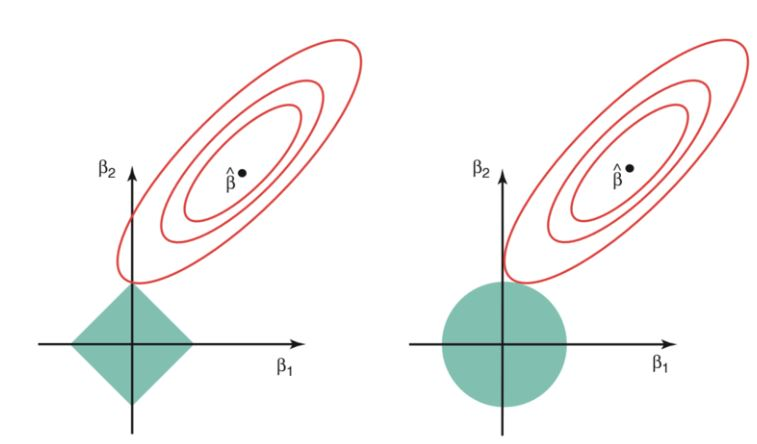
\includegraphics[width=0.56\textwidth]{images/ch1/L1_vs_L2.JPG}
    \caption{Solution space of the lasso (left) and ridge regularization (right). Original image from \cite{generic_stats}.}
    \label{fig:01l1vsl2}
\end{figure}   

Two other popular, but specialized regularization techniques catered towards neural networks are drop-out and batch normalization \cite{dropout, batch_norm}. Figure \ref{fig:01dropout} shows a neural network with and without drop-out. On a high level, drop out randomly disable neurons during training to prevent major "co-adaptation" between adjacent neurons. Intuitively, the drop-out process introduces (significant) pseudo noise into the training step, forcing neurons to learn a more probabilistic mapping. Ultimately, the drop-out method was able to achieve state-of-the-art performance when tested on various data sets in computer vision, natural language processing, classification, and computational biology. A more detailed explanation of drop-out can be found in \cite{dropout}.   

\begin{figure}[H]
    \centering
    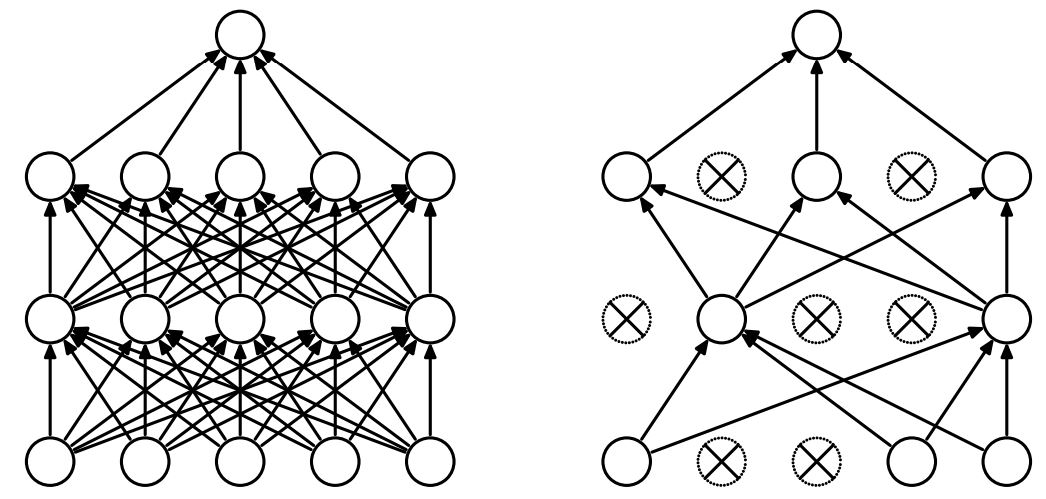
\includegraphics[width=0.56\textwidth]{images/ch1/dropout.jpg}
    \caption{A neural network with (right) and without (left) drop-out \cite{dropout}.}
    \label{fig:01dropout}
\end{figure}  

Batch normalization is another recently popularized regularization method in deep learning.  Neural networks are trained through backpropagation.  In this method, the accuracy of the neurons in the later layers are paramount for proper parameter updates in the earlier layers.  If not, the backpropagated errors are significant incorrect. Specifically, the distribution of different layer's inputs change during training due to the weight changes of the subsequent layers. This characteristic, called internal covariate shift, contains a significantly negative effect on the training time of neural networks.  Batch normalization aims to overcome internal covariate shift by normalizing layer inputs.  In doing so, deep neural networks are less sensitive to initializations and much larger learning rates can be used. Additionally, the method was shown to contain regularization effects and often times eliminate the need for drop-out.  In experiments, the authors found that neural networks using batch normalization can achieve previous accuracies with 14 times fewer training steps.  For more information on batch normalization, see \cite{batch_norm}.


%%%%%%%%%%%%%%%%%%%%%%%%% End Section Function Approximation %%%%%%%%%%%%%%%%%%%%%%%%%%%%%%%


%%%%%%%%%%%%%%%%%%%%%%%%%%%%%%%%% Begin Section DDPG %%%%%%%%%%%%%%%%%%%%%%%%%%%%%%%%%%%%%%%

\section{Deep Deterministic Policy Gradient}
Deep deterministic policy gradient was introduced as one of the first RL architectures to handle both continuous states and continuous actions \cite{ddpg}. Additionally, it was shown to also work in massively large state and action space systems (one such system was $x \in R^{102}$ and $u \in R^{9}$). DDPG contains four neural networks and employs an actor-critic framework.  The actor is the deterministic policy gradient (DPG) algorithm and maps states to actions.  Similarily, the critic is the deep $Q$-learning network (DQN) algorithm and approximates the action-values of the state-action pairs. Intuitively, combining DPG and DQN into one unifying algorithm overcomes several shortcomings exhibited by each algorithm individual. For example, policy gradients were traditionally trained using MC methods and cannot update mid-episode; however, DDPG trains the DPG using the gradient of the DQN, allowing for inter-episode updates. Furthermore, DQN cannot output continuous actions, but DDPG can by leveraging DPG to select actions.  Another advantage provided by DDPG is the mitigation of large variances in the DPG through the use of DQN.  Previously, DPG experiences high variance because similar action sequences may return different outcomes in stochastic environments; however, evaluating the action using the DQN (a deterministic function) will result in an unbiased estimate of performance \cite{ddpg}.  

\subsection{Actor - Deterministic Policy Gradient}
The DDPG leverages the DPG algorithm to deterministically map \textit{continuous} states to \textit{continuous} control actions.  Classically, policy gradient algorithms represent the policy as a probability distribution $\pi_{\theta}(u|x) = \mathbb{P}[u|x; \theta]$ which stochastically maps states to actions \cite{dpg}.  In DPG, \textit{deterministic} policies are considered instead and are given by $u = \mu_{\theta}(x)$. Comparatively, deterministic policies are more advantageous because only $Q^{\mu}(x, \mu_{\theta}(x))$ is required during updates steps compared to $\sum\limits_u \pi(u|x)Q^{\mu}(x, u)$. Here, $\pi(u|x)$ denotes the probabilities of picking different actions $u$ in $x$.

Like all experience driven RL algorithms, exploration is required in DPG; thus, requiring some stochastic behaviour policy (ironically making it non-deterministic). To this end, DPG can be trained using an \textit{off-policy} actor-critic method where a deterministic policy is identified while following a separate exploratory policy.  Such a concept is analogous to $Q$-learning, where a deterministic greedy policy is identified while following a noisy behaviour policy (typically $\epsilon$-greedy) during training. For a detailed explanation of DPG, please refer to \cite{dpg}.


\subsection{Critic - Deep Q-learning Network}
In DDPG, DQN is used to reduce variance and provide off-policy training to the DPG. DQN is a deep $Q$-learning approach to map from states to action-value functions \cite{dqn1, dqn2}. Historical methods to train deep $Q$-learning were unstable and data inefficient. Authors of DQN introduced two important concepts in the DQN algorithm---the experience replay and target networks---to significantly improve convergence rate. The \textit{experience replay} is a dictionary of tuples $(x, u, r, x')$.  During training, random mini-batch of experience tuples are sampled to enhance data efficiency (same experiences used many times) and to provide the agent with temporally de-correlated training examples. The target network solves the "moving target problem".  In all deep $Q$-learning approaches, supervised learning models are used to predict for the action-values.  Initially, the model is trained using:
\begin{equation}
    y_i(x, u, r, x') = r + \gamma \max_u Q_{\theta}(x', u')
    \label{eq:01tdtarget}
\end{equation}
\begin{equation}
    J(\theta) = \mathbb{E}_{(x, u, r, x') \thicksim U(R)}\left[(y_i - Q_{\theta}(x, u))^2     \right]
\end{equation}
where $Q_{\theta}$ denotes the predicted $Q$ value given model parameters $\theta$.  Additionally, $(x, u, r, x') \thicksim U(R)$ represents sampling experience tuples from the experience replay following an uniform distribution and $y_i$ denotes the "target" $Q$ value (i.e., the label to the model). From Equation \label{eq:01tdtarget}, $y_i$ is also partly calculated from the $Q$ value prediction model. As the model updates, $y_i$ will consistently change, creating an ill-posed minimization problem ultimately resulting in poor learning.  In DQN, a \textit{target network} is introduced to prevent this problem.  Architecturally, the target network is an exact copy of the original model; however, the model weights are a time-delayed version of the "online" model.  That is, the weights of the target network are kept constant for a period of time and are used to compute $y_i$.  By doing this, the target (although inaccurate during initial episodes) remains stationary during the optimization step.  After a period of time, the target network copies the weights from the online model and the procedure is repeated until accurate $Q$-values can be predicted.  Typically, this occurs when the target and online network are sufficiently similar.

A more detailed explanation of experience replay is provided below.  For complete details, see \cite{exp_replay, p_exp}. For more details the target network or DQN, see \cite{dqn1, dqn2}.  

\subsection{Exploration in DDPG}
Traditionally, exploration in continuous action spaces are difficult because classical approaches, such as $\epsilon$-greedy, work only in a discrete action space.  DDPG explores through corrupting the action with exploratory noise \cite{ddpg}.  Throughout RL literature, many researchers conduct exploration using white noise. The noise corrupted action is given by:
\begin{equation}
    u'(x_t) = u(x_t|w_t) + \mathcal{N}
    \label{eq:01noise_corrupt}
\end{equation}
where $u'(x_t)$ is the action corrupted by some noise, $\mathcal{N}$.

\subsubsection{Exploration using White Noise}
In Equation \ref{eq:01noise_corrupt}, $\mathcal{N}$ can be white noise drawn from $\mathcal{N}(0, \sigma^2)$; however, white noise is de-correlated and is ineffective for "deep" exploration (i.e., traversing far from the current state) due to the zero averaging effect \cite{white_noise}. Intuitively, white noise simply introduces oscillation into the process and does not create displacement in any particular direction. Therefore, it is more effective to corrupt the action using a temporally correlated process such as the Uhlenbeck-Ornstein (UO) process.

\subsubsection{Ornstein-Uhlenbeck Exploratory Noise}

The UO process is given as \cite{ornstein}:
\begin{equation}
    dx_t = \theta x_t dt + \sigma dW_t,
    \label{eq:01OU}
\end{equation}
where $\theta > 0$, $\sigma > 0$, and $W_t$ denotes the Wiener process. Mathematically, the Wiener process is a special case of a continuous time stochastic process. Detailed information regarding the Wiener process and its properties can be found in \cite{wiener}. The UO process is ideal for exploratory noise in RL because of its time correlated feature.

Intuitively, actions $u_t$ from the RL agent can be understood as exerting an external force upon physical bodies and is given by \cite{physics}:
\begin{equation}
    u = m \ddot{x}
\end{equation}
where $m$ and  $\ddot{x}$ denotes mass and acceleration, respectively.  To obtain displacement (i.e., movement in the state space), the force must be integrated twice:
\begin{equation}
    x = \frac{1}{m}\int \int u
\end{equation}
Interestingly, integration operators are low-pass filters and will remove high frequency noise contained in $u$ that are generated by the Wiener process \cite{process_control_ref13}. Consequently, this results in smooth displacements in temporally correlated processes, such as the UO process.  Additionally, the displacement will typically stay in the same direction for long durations, allowing for deep exploration the state space. For example, Figure \ref{fig:01OU} shows the trajectory of a randomly generated OU process, and its corresponding effect on the displacement of the agent inside the state space.  It can be seen that the displacement is smooth and is heavily biased towards one direction, ultimately promoting deep exploration.

\begin{figure}[H]
    \centering
    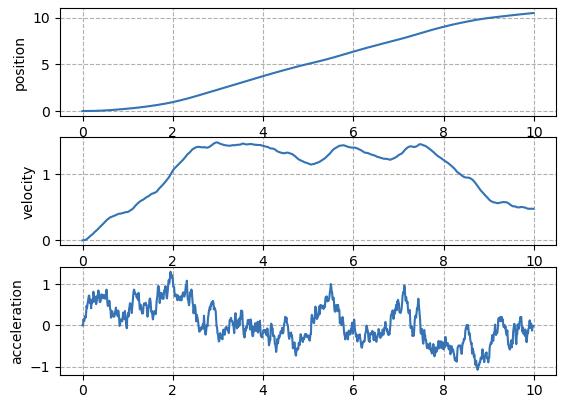
\includegraphics[width=0.56\textwidth]{images/ch1/01OU.jpeg}
    \caption{Change in displacement caused by a randomly generated OU process.}
    \label{fig:01OU}
\end{figure}   


\subsection{Stabilization of Training}
Architecturally, DDPG contains two interacting neural networks that are trained upon each other.  To successfully train such a complicated system, careful parameter initialization and proper weight updates are paramount.  Although some initialization techniques were introduces in the above sections, the authors of \cite{ddpg} initiated the last layer of the networks with weights uniformly drawn from $[-3 \times 10^{-3}, 3 \times 10^{-3}]$ for low dimensional problems. Such an initialization ensures initial policy and value estimates were near zero \cite{ddpg}. The other layers were initialized using uniform distributions $[-\frac{1}{\sqrt{n_j}}, \frac{1}{\sqrt{n_j}}]$, where $n_j$ was the size of the previous layer.  Regularization-wise, batch normalization was used \cite{batch_norm}. For exploration, the UO noise given in Equation \ref{eq:01OU} with $\theta$ and $\sigma$ as 0.15 and 0.2 was used.

\subsubsection{Experience Replay}
DDPG also uses experience replay (sometimes called replay buffer) to enhance data efficiency and prevent catastrophic interference during training.  Experience replay was first introduced in \cite{exp_replay} to provide temporally de-correlated training samples to agents in time-series settings. In DDPG, tuples of:
$$(x_t, u_t, r_{t+1}, x_{t+1})$$
are memorized and stored in the experience replay. During updates, random mini-batches of previous experiences are sampled from the replay buffer to update the agent. Consequently, the agent obtains the ability to learn the same experiences many times, a concept similar to cycling through many epochs in deep learning. Correlating to humans, experience replay is similar to hippocampal replay, where memories are sub-consciously replayed over and over.  Indeed, that is one theory explaining the efficiency of human learning \cite{hippocampal}. However, human memories are rarely replayed randomly. Instead, only the most important or unexpected memories are replayed. Prioritized experience replay mimics this concept and biases sampling to experiences with large TD errors \cite{p_exp}. Intuitively, such experiences are \textit{shocking} since the outcome was significantly different than what was expected. Using prioritized experience replay, the agent learned faster in 41 out of 49 ATARI games compared to the original experience replay.

\subsection{Input and State Constraints}
As with all RL methods, input constraints can be handled quite trivially; however, state constraints are much more difficult. Typically, \textit{soft} state constraints are implemented in RL by introducing large negative rewards when the agent arrives at an undesired states. Indeed, humans learn state constraints in such a way where guardians provide negative consequences when we venture into troubling situations.  In literature, constrained Markov decision processes (CMDPs) and safe RL are two fields that explore how RL can handle constraints explicitly; however, most modern methods either require explicit system models or are difficult to implement in industry. 


\subsection{Training Algorithm}
The DDPG algorithm is trained as follows \cite{ddpg}:
\begin{enumerate}
    \item Initialize replay buffer and the actor and critic network weights corresponding to the previous subsection.
    \item Observe some states from the system 
    \item Map the states to some exploratory actions via the online actor network: $$\mu_t' = \mu (x_t | \theta ^{\mu}) + \mathcal{N}_t$$
    \item Implement $\mu_t$ to the system, observing transition to $x_{t+1}$ and obtaining $r_{t+1}$
    \item Store tuple $(x_t, \mu_t, r_{t+1}, x_{t+1})$ into the replay buffer
    \item Sample a mini-batch of $N$ experiences $(x_t, \mu_t, r_{t+1}, x_{t+1})$ from the replay buffer
    \item Using the target critic network, compute $y_t = r_t + \gamma Q'(x_{t+1}, \mu'(x_{t+1}|\theta^{\mu'})|\theta ^{Q'})$ for each experience
    \item Update online critic parameters by minimizing: $J = \frac{1}{N}\sum(y_i - Q(x_t, u_t|\theta^{\mu}))^2$
    \item Update online actor parameters by:
    $$\nabla_{\theta^{\mu}} J \approx \frac{1}{N}\sum \nabla_u Q(x, u|\theta^Q)|_{x = x_t, u = u_t}\nabla_{\theta^{\mu}}\mu (x | \theta^{\mu})|_{x_t}$$
    \item Update both actor and critic target networks:
    $$\theta^{Q'} \leftarrow \tau \theta^Q + (1 - \tau) \theta^{Q'}$$
    $$\theta^{\mu'} \leftarrow \tau \theta^{\mu} + (1 - \tau) \theta^{\mu'}$$
\end{enumerate}

Most steps above are intuitive to understand; however, steps 6 and 9 might be slightly confusing. In step 6, mini-batches of experiences are used for training to enhance data efficiency and to provide temporally de-correlated training data.  For time-series problems, such as continuous control, a direct adaptive control method like RL will quickly adapt to the current operating condition and exhibit catastrophic interference on other operating conditions.  By training on an uniformly sampled mini-batch of historical experiences, catastrophic interference can be largely avoided.

Step 9 shows the slow update of the actor and critic target networks.  This follows the same intuition as DQN, where the target network is frozen for periods of time to prevent the moving target problem.  Except in DDPG, the target networks are updated in small steps after each episode rather than being kept frozen, and then undergoing a complete update.



%%%%%%%%%%%%%%%%%%%%%%%%%%%%%%%%%% End Section DDPG %%%%%%%%%%%%%%%%%%%%%%%%%%%%%%%%%%%%%%%%



% %%%%%%%%%%%%%%%%%%%%%%%%%%%%%%%%%%%%%%%%%%%%%%%%%%%%%%%%%%%%%%%%%%%%%%%%%%%%%%%%%%%%%
% % Model Predictive Control
% %%%%%%%%%%%%%%%%%%%%%%%%%%%%%%%%%%%%%%%%%%%%%%%%%%%%%%%%%%%%%%%%%%%%%%%%%%%%%%%%%%%

% %%%%%%%%%%%%%%%%%%%%%%%%%%%%%%%%%%%%%%%%%%%%%%%%%%%%%%%%%%%%%%%%%%%%%%%%%%%%%%%%%%%%%
% Model Predictive Control
%
%
%
%
%%%%%%%%%%%%%%%%%%%%%%%%%%%%%%%%%%%%%%%%%%%%%%%%%%%%%%%%%%%%%%%%%%%%%%%%%%%%%%%%%%%

\section{Model Predictive Control}

Compared to all topics in process control, the concepts of model predictive control (MPC) is perhaps the closest resemblance to modern RL.  MPC is a model-based control strategy (known as a planning method in RL literature) that optimizes the input trajectory of a system by using the functional equation (a function where the unknowns are also functions) generated from the system's state information together with a value function. The performance of MPCs heavily rely on the accuracy of system identification as the input trajectory is solved by extremizing an objective function using mathematical programming (MP) as a function of the process model \cite{mpc}. The objective function is typically given as:
\begin{equation}
    J = \sum\limits^{N}_{i = 1} x_i^TQx_i + \sum\limits^N_{i=1}u_i^TRu_i
    \label{eq:mpc_cost}
\end{equation}
where $N$, $Q$, and $R$ are the prediction horizon and tuning matrices, respectively. Superscript $T$ denotes the transpose operation. $Q$ and $R$ are diagonal matrices and are used to emphasize importance on different state and inputs, respectively. Here, $x$ and $u$ are given as:
\begin{equation}
    x_{sp} - x_i
\end{equation}
\begin{equation}
    u_{ss} - u_i
\end{equation}
where subscripts $sp$ and $ss$ denote the set-point and steady state, respectively. Often times in optimal control, $u_{ss}$ is unknown. In such scenarios, $u$ is given as $\Delta u$ instead, representing a cost in changing the inputs at each step.

Implementation-wise, MPC uses a receding horizon approach where the controller predicts and optimizes for a set amount of steps into the future.  However, only the first control action is implemented.  During the next sampling time, the trajectory is re-optimized and the cycle repeats. The length of the input trajectory and the number of steps the controller predicts into the future are known as the control and prediction horizon, respectively. During design, it is paramount to ensure that both the prediction and control horizons are adequate in length to ensure global optimal solutions.  Intuitively, the prediction and control horizon can be related to the everyday task of driving a car.  It would be very dangerous if we only consider events one second into the future because it would be difficult to react to curves and other road side disturbances; therefore, the prediction and control horizons must be sufficiently long to ensure safe and optimal driving practices. Typically, the control horizon is chosen to be shorter than the prediction horizon due to computational cost and the unimportance of unnecessarily long input trajectories \cite{prediction_horizon}.  One flaw with the receding horizon approach is its extremely expensive online computational cost, especially in large non-linear systems.  

Explicit MPC was developed to mitigate this computational burden by leveraging parametric programming to pre-compute solutions to the optimization problem offline \cite{explicit_MPC}.  During online evaluation, the controller simply looks up the optimal input from a dictionary of pre-computed solutions, making online evaluation extremely fast. This idea is exactly equivalent to RL, where the agent is trained offline (i.e., solves the optimal policies offline), allowing extremely fast online evaluations. 

Ultimately, MPCs provide many advantages compared to classical control strategies.  For example, MPC considers long term planning and identifies the optimal input trajectory rather than the best immediate action.  Furthermore, MPCs have predictive capabilities and can anticipate future events, allowing the controller to plan future control actions accordingly.  A third advantage is that the MP methods used in MPC have been widely demonstrated to handle both input and state constraints relatively successfully.  In modern times, MPCs are often implemented in the supervisory control layer.

The process control hierarchy is shown in Figure \ref{fig:rto_mpc_pid}. Starting from the bottom, the \textit{regulatory controllers} are typically used to ensure stability of the process and directly actuate the process instrumentation.  A common regulatory controller is the Proportional-Integral-Derivative controller (PID). The layers above are known as the \textit{supervisory controllers}. MPC is a common supervisory controller and is classically implemented for regulation or set-point tracking problems exclusively.  Economic objectives of the process were managed by the real time optimization (RTO) layer through steady state optimization \cite{rto}. More recently, control practitioners began to unify the ideas of RTO and MPC into a centralized algorithm called economic model predictive control (EMPC).  Here, the economic objective of the RTO is placed into the objective function of the MPC, allowing for the input trajectory to optimize the economic objective instead \cite{empc2, empc1}. 

\begin{figure}[H]
    \centering
    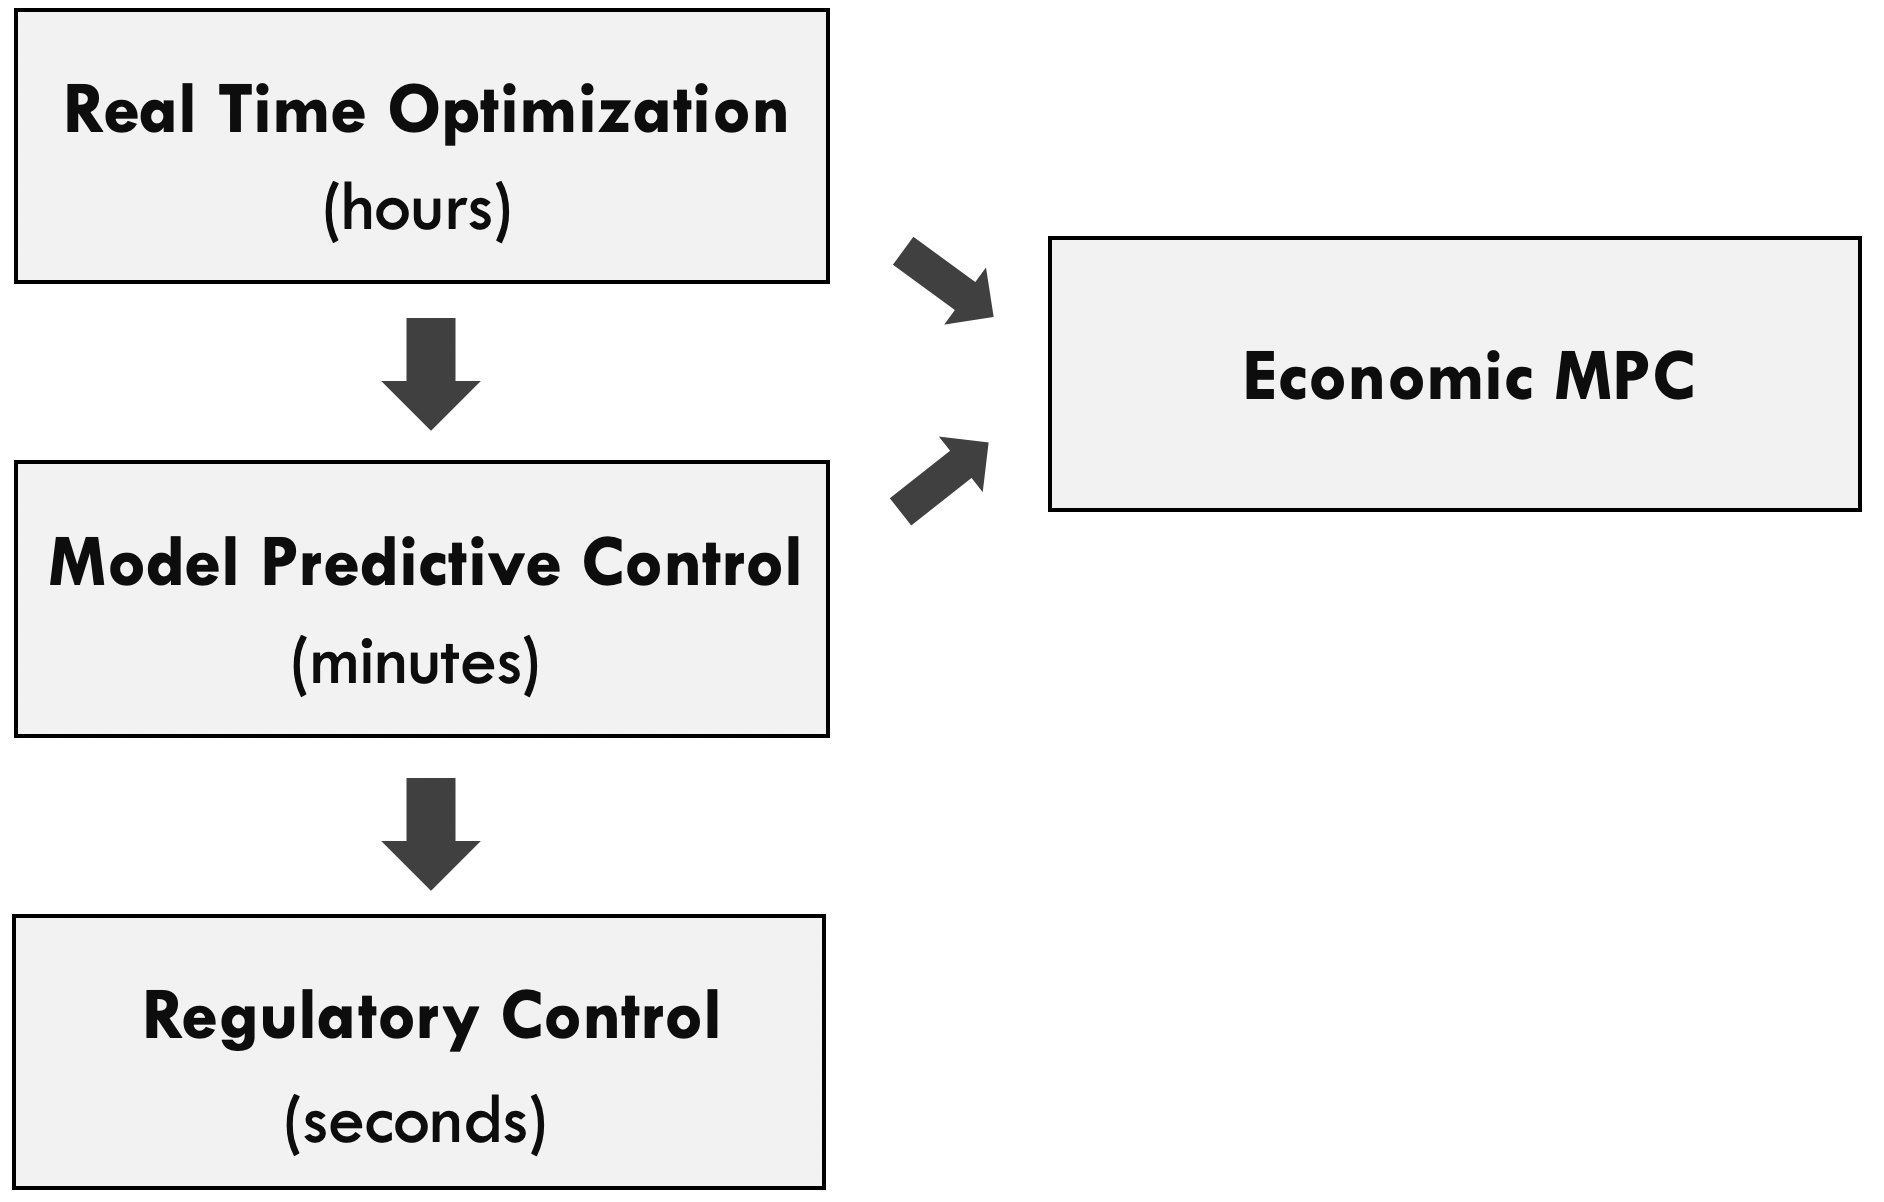
\includegraphics[width=0.5\textwidth]{images/ch1/rto_mpc_pid.jpeg}
    \caption{A typical industrial control architecture.}
    \label{fig:rto_mpc_pid}
\end{figure}

Comparatively, RL can be described as a general control algorithm and can be used to replace \textit{any} layer in Figure \ref{fig:rto_mpc_pid}. For example, a MPC or PID based RL would have its reward function to be identical as the negative of Equation \ref{eq:mpc_cost}.  In the EMPC case, the reward function of RL would instead be the economic objective.  In Chapter 4, the performance of RL based supervisory controls will be extensively compared to traditional methods on simple and complicated processes. Additionally, the pros and cons of each method will be summarized.
